\label{detbeamtest}

The primary goals of DUNE are to 
constrain or discover CP violation in the lepton sector by determining 
the value of the
CP violating phase, $\delta_{CP}$, and
to determine the mass ordering of the three neutrino mass eignestates. 
This will be accomplished through measurement of 
the appearance rate of electron neutrinos and electron anti-neutrinos 
as well as the corresponding disappearance rate of muon neutrinos 
and muon anti-neutrinos over the 1300~km baseline of the experiment. 
Other important physics goals include sensitive searches for proton decay (PD) and detection of supernova neutrinos.

The full power of the DUNE experiment to perform a careful test of the three-flavor paradigm will come from a measurement of the detected neutrino spectral shape over a broad energy range.  For a baseline of 1300 km the first maximum of the oscillation probability occurs around 2~GeV and the second oscillation maximum is around 0.6~GeV,
 so the high intensity neutrino flux must be maximized in the energy range from 0.5 - 5~GeV. It is desirable to have sufficient flux in the sub-GeV energy range to enable a measurement of the rapidly changing spectral shape in the region of the second maximum in the oscillation probability. It is this requirement on the neutrino energy spectrum, and the subsequent energy range of charged particles that result from their interactions, that determines the performance requirements for the DUNE detectors. 


One of the main goals of DUNE-PT test beam program is to perform measurements 
needed to control and understand systematic uncertainties in DUNE oscillation measurements.
%The program also includes measurements to support other important DUNE physics measurements as described below.
%detector is intended to provide input necessary to reduce systematic uncertainties for oscillation measurements 
As an example of the importance of controlling detector related uncertainties,
Fig.~\ref{fig:spectraleffect} shows the effect of a reconstructed neutrino energy scale 
shift of -5\% on the measured 
appearance signal %(for $\delta_{CP}=0$)
 and backgrounds in DUNE. 
The expected signal shape is shown for several values of $\delta_{CP}$. 
%(solid curve: $\delta_{CP}=0$, lower crosses: $\delta_{CP}=+\pi/2$, and upper crosses: $\delta_{CP}=-\pi/2$). 
Energy scale uncertainties will distort and shift the $\nu_e$ appearance spectra and
can mimic a non-zero
$\delta_{CP}$ phase.
\begin{figure}[h!]
\centering
%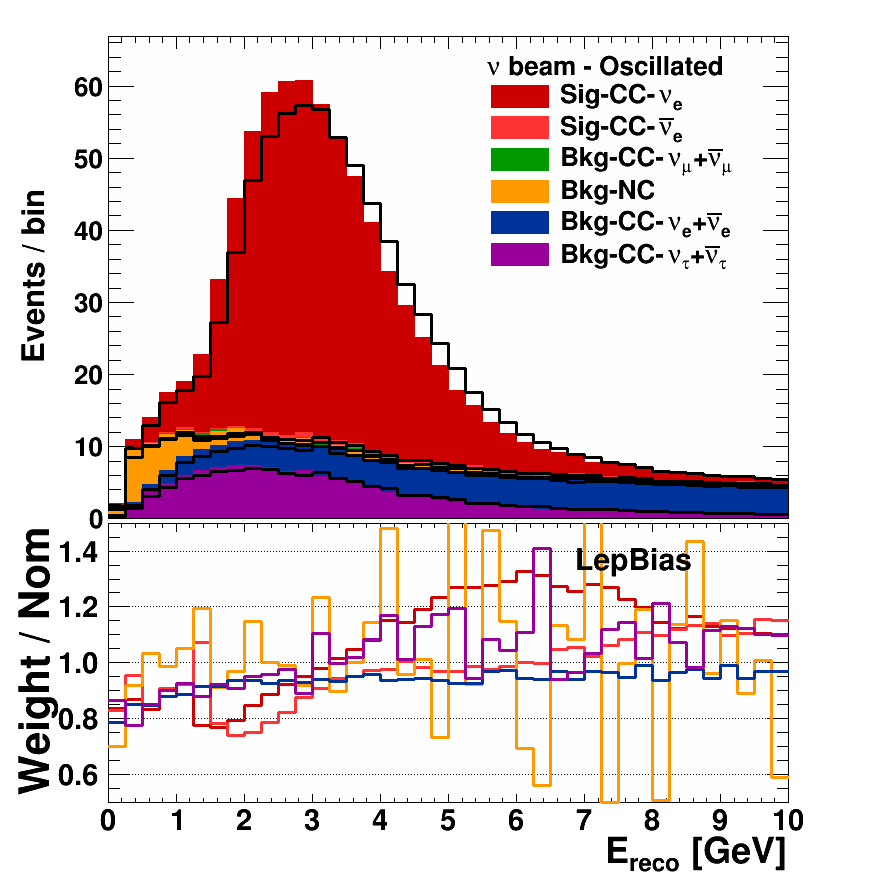
\includegraphics[width=0.7\textwidth,height=7.7cm]{figures/lepbias10}
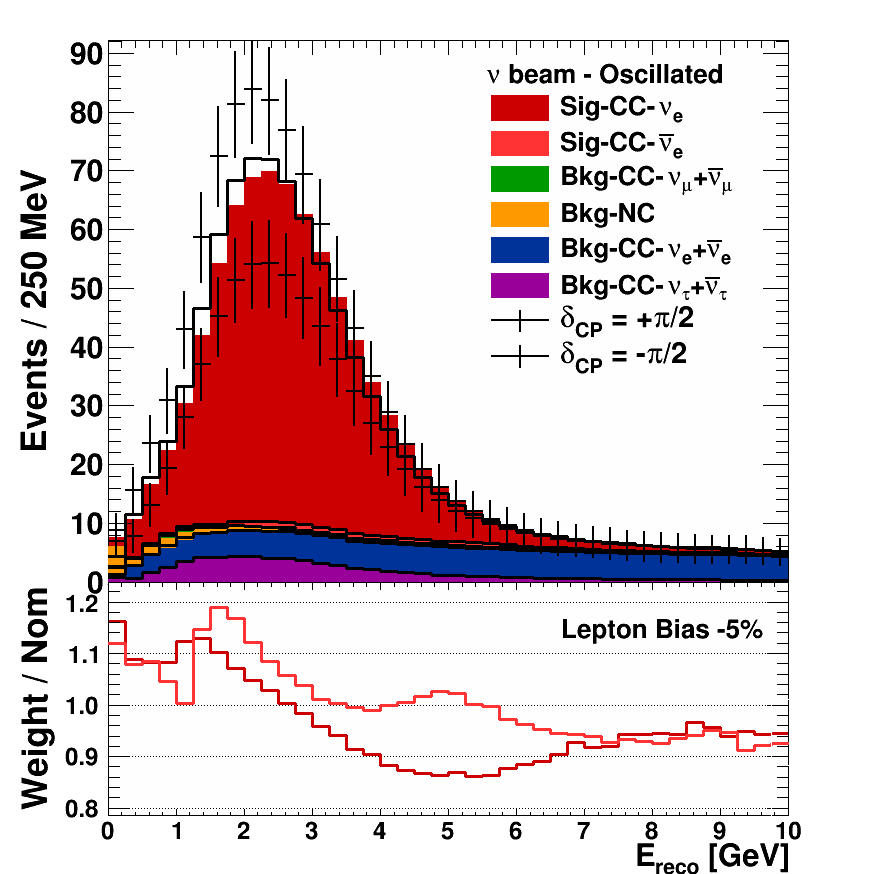
\includegraphics[width=0.7\textwidth,height=7.7cm]{figures/CSPP_LeptonBias_nue_app_FHC}
  \caption{DUNE $\nu_e$ appearance signal and background spectra. 
Solid curves show the effect of -5\% reconstructed neutrino energy scale shift on the 
measured appearance $\nu_e$ and $\overline{\nu}_e$ signals assuming $\delta_{CP}=0$.
The crosses show the expected signal shape for $\delta_{CP}=+\pi/2$ (lower crosses) and -$\pi/2$  (upper crosses). 
Ratios show the distortion on the $\nu_e$ and $\overline{\nu}_e$ spectra due to the 
5\% energy scale shift.
}
\label{fig:spectraleffect}
\end{figure}


 Fig.~\ref{fig:global_escale_sens} taken from \cite{dunecdr} demonstrates that
energy scale uncertainties will impact DUNE 
%shows the effect of 
%three values of neutrino energy scale uncertainty on the DUNE 
mass hierarchy (left) and $\delta_{CP}$ (right) sensitivities.
%The exposure to achieve this level of sensitivity corresponds to 
%The nominal sensitivity assumes a
% 230-400 kt-MW-years for mass hierarchy and  850-1320 kt-MW-years for CPV depending on the 
%115 kt-MW-years in each of neutrino and anti-neutrino modes.
%The sensitivities will also depend on the
%details of the LBNF neutrino beam design.
%exposure with equal neutrino and antineutrino running. 
Work to evaluate the effect of all systematic uncertainties in DUNE sensitivities is still in progress.
This study already indicates a significant reduction of the CPV peak sensitivity due to a reconstructed neutrino energy scale uncertainty. 
This example assumes linear neutrino energy scale variations at the levels indicated.
More complex (and more likely) scenarios for energy scale uncertainties are under study and
will likely result in larger effects on the sensitivities.
%including separate particle
% correlated variations 
%It therefore likely underestimates the probable effects  of particle energy reconstruction 
%on DUNE sensitivities.
%The size of effects shown here do not account for correlated uncertainties in neutrino and 
%antineutrino running or effects on backgrounds and is therefore likely
%a best-case scenario. 
\begin{figure}[h!]
\centering
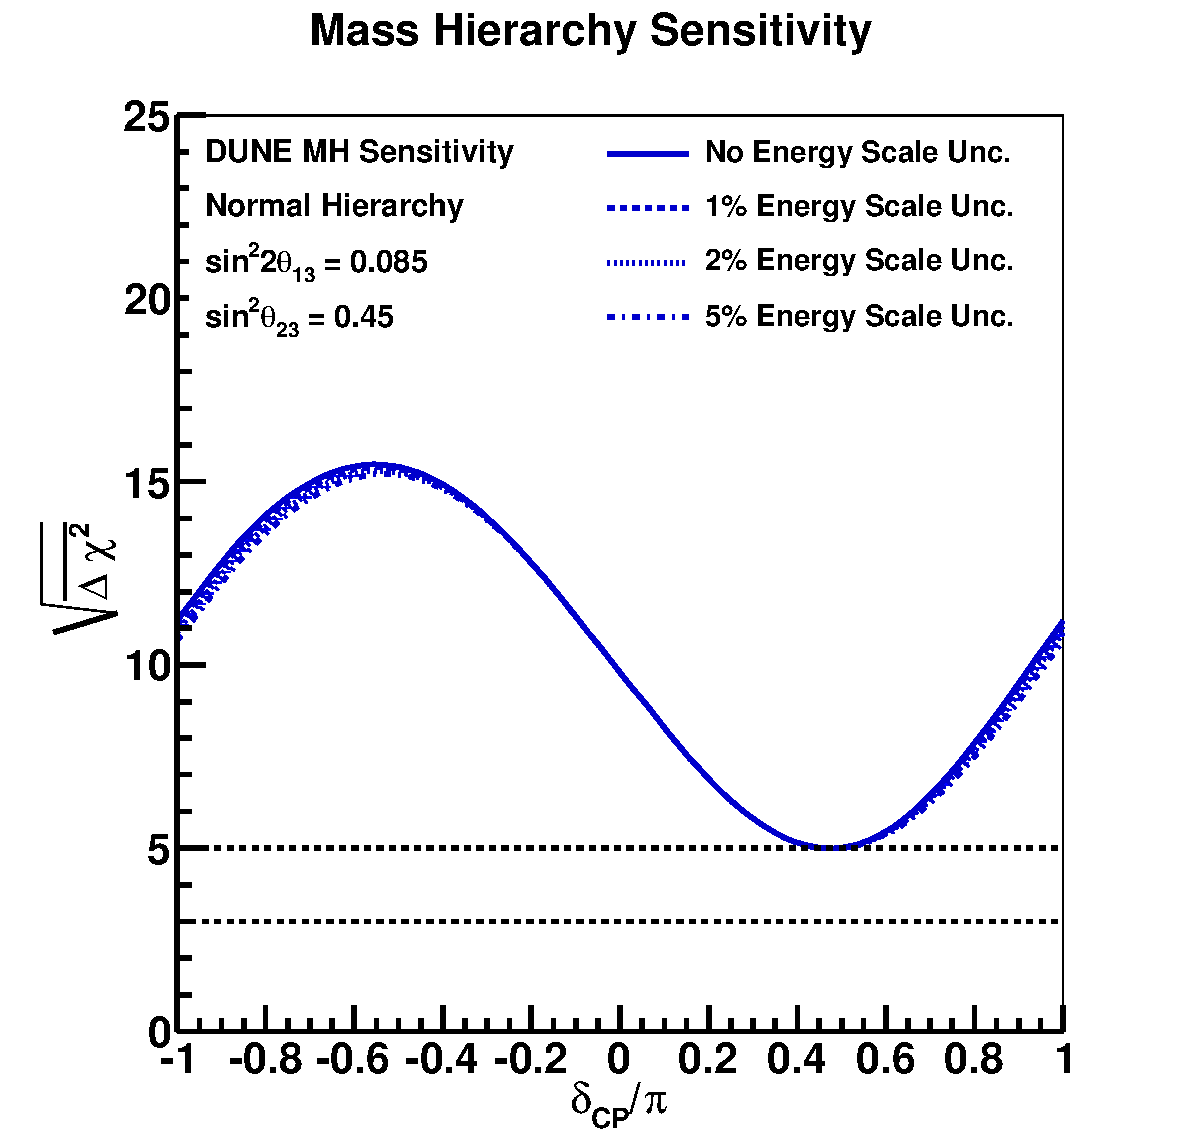
\includegraphics[width=0.49\textwidth,height=6.7cm]{figures/mh_230ktmwyear_varyesyst}
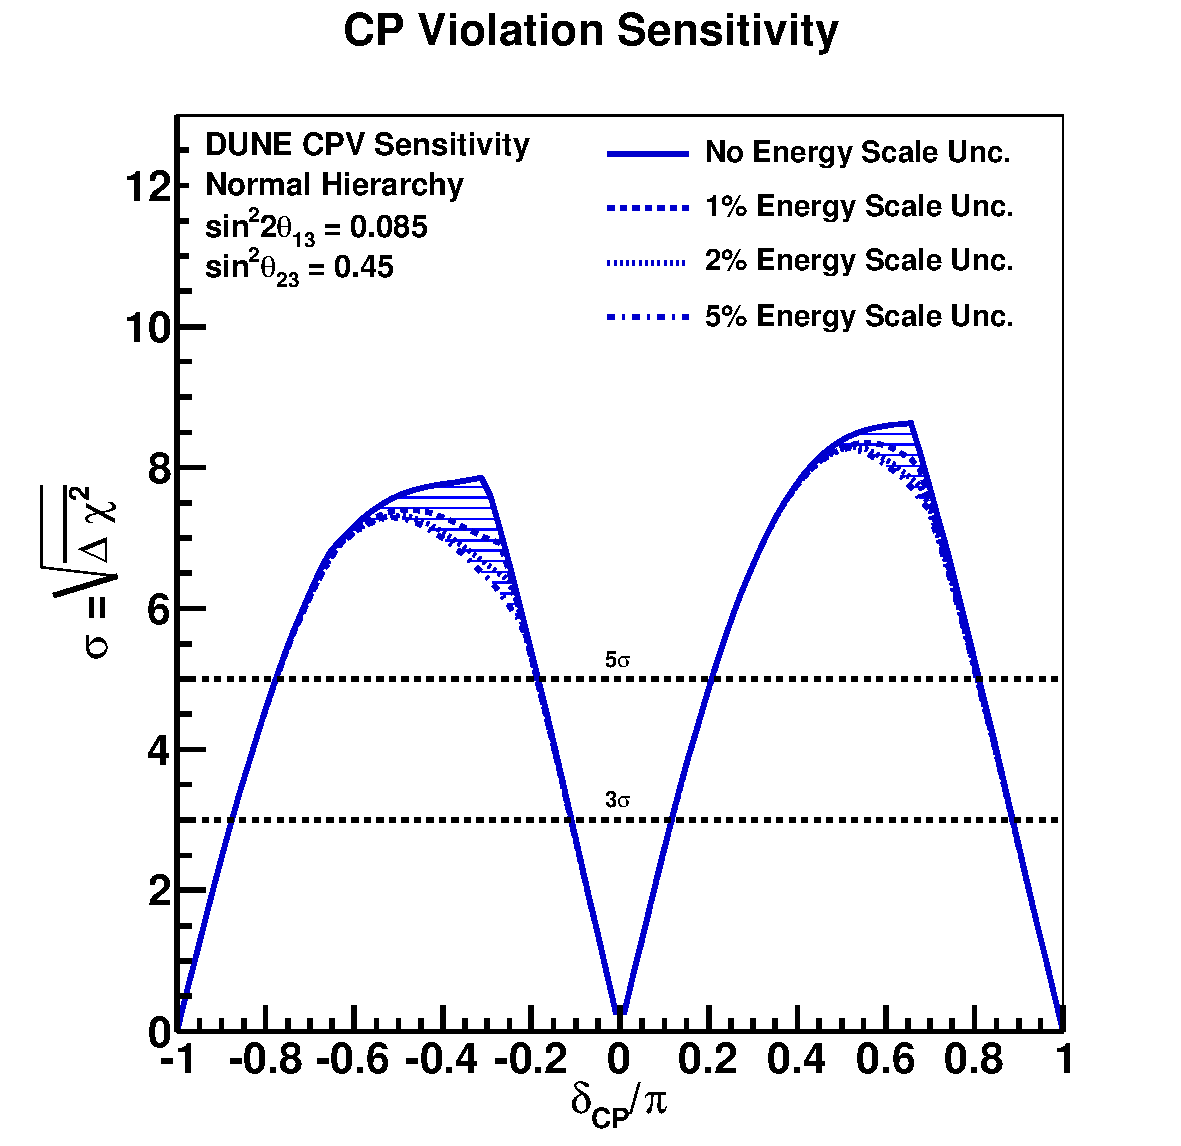
\includegraphics[width=0.49\textwidth,height=6.7cm]{figures/cpv_890ktmwyear_varyesyst}
%\includegraphics[width=0.49\textwidth,height=6.7cm]{figures/mh_escale_sens}
%\includegraphics[width=0.49\textwidth,height=6.7cm]{figures/deltacp_escale_sens}
  \caption{One scenario for the effect of 1-sigma  neutrino energy scale uncertainties on
DUNE projected sensitivity for mass hierarchy (left) and $\delta_{CP}$ 
(right).  In the left figure, the beam conditions are chosen so that the case with no energy scale systematic provides a significance of at least 5$\sigma$ for all values of $\delta_{CP}$. In the right figure, the beam conditions are chosen so that the case with no energy scale systematic provides a significance of at least 3$\sigma$ for 75\% of $\delta_{CP}$ values.  Sensitivities are for true normal hierarchy; neutrino mass hierarchy and $\theta_{23}$ octant are assumed to be unknown.
% to one sigma neutrino energy scale uncertainties as indicated.
%If energy scale uncertainties can be controlled at the appropriate levels, DUNE can achieve 
%at least 5$\sigma$ sensitivity on mass hierarchy determination for 100\% of $\delta_{CP}$ values and
%for 3$\sigma$ sensitivity to  $\delta_{CP}$ for 75\% coverage of phase space.
}
\label{fig:global_escale_sens}
\end{figure}

%Current levels of sensitivity in ~\cite{dunecdr} assumes
%$\nu_e$ energy scale is known at the level of 2\%. 
%More here...
%will require a dedicated test beam


%$\nu_e$ energy scale  & 2.7\% & 2.5\% & 2\% & comment \\ \hline
%\end{tabular}


\subsection{Detector and beam requirements }
\label{detbeam_main}

LAr TPC technology was first proposed for use in neutrino experiments by C. Rubbia in 1977
\cite{CRubbia} but extensive use in neutrino experiments is only now being realized. 
%CERN-EP-INT-77-8
%Title 	The liquid-argon time projection chamber : a new concept for neutrino detectors
%operating in the CNGS beamline  (with mean beam energy $\sim$17 GeV)~\cite{ICARUSmain}. 
The ICARUS T600 detector~\cite{icarus_mainref} pioneered the first large-scale detector when it operated in the CNGS 
neutrino beam at mean energy of $\sim$17 GeV. ArgoNeuT~\cite{argoneut1}\cite{argoneut2} recently studied 
neutrino interactions in the NuMI beam down to sub-GeV energies with a small-scale (175~L fiducial volume) detector. 
While these samples are proving useful, they do not allow full isolation of
the low energy neutrino interaction processes
and final states from reconstruction and detector effects. 
The use of this technology in future precision neutrino experiments will require dedicated 
information on particle response
in the sub-GeV to few-GeV range provided by charged-particle test beams. 

%%%
%\subsubsection{Particles energy and direction}
%\label{detbeam_particles}
The DUNE experiment will run in both neutrino and anti-neutrino 
configurations. These beams will be composed  mainly of muon neutrinos (anti-neutrinos) as well as electron neutrinos (anti-neutrinos). In Fig.~\ref{fig:particle_momenta} the distributions of momenta and angles of particles created in neutrino interactions from 
simulated beam fluxes, including oscillation effects, are shown. The particle rates are normalized  to the number of neutrino interactions in the DUNE far detector and to the neutrino beam flux.
% In addition the electron rates from charged current interactions for muon neutrinos oscillated to electron neutrinos are shown. 
\begin{figure}[h!]
  \centering
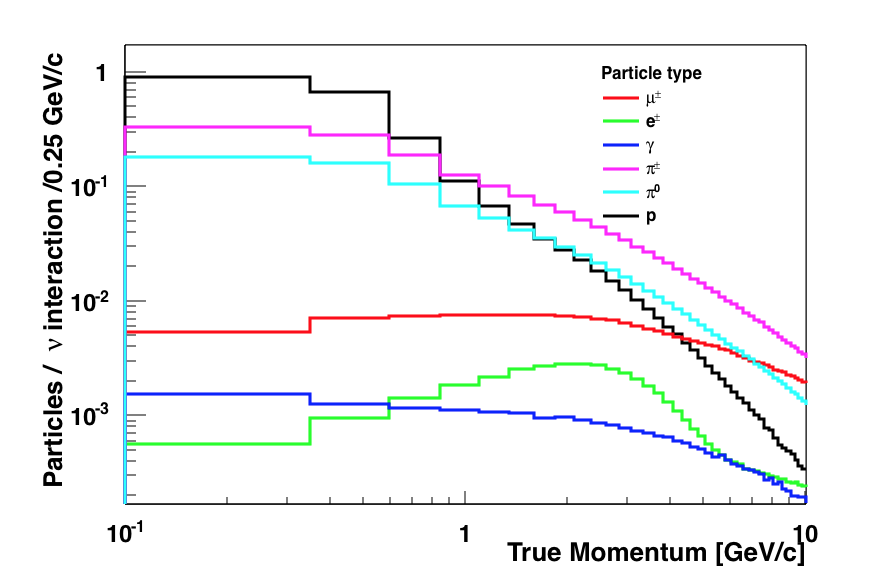
\includegraphics[width=0.49\textwidth,height=6.0cm]{figures/True_Momenta_per_Particle_9_2_1_0_logy_logx} 
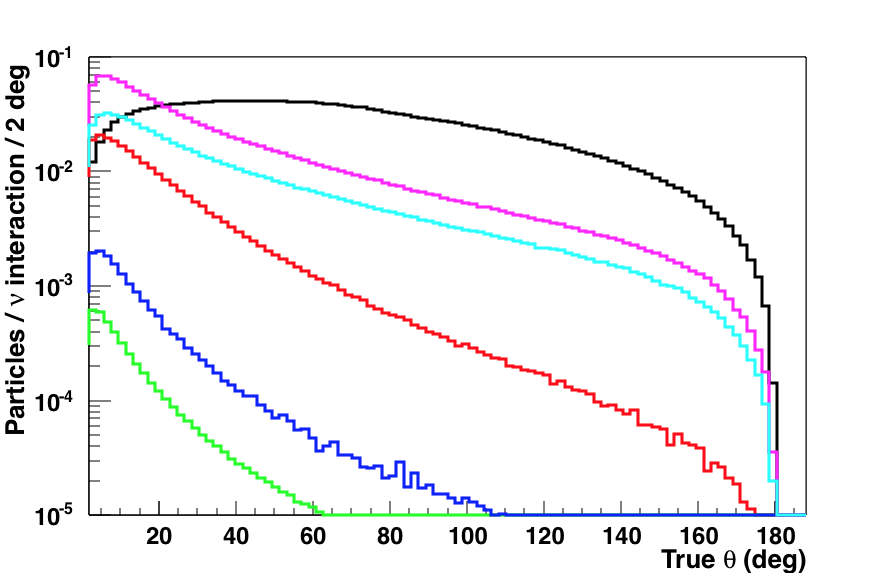
\includegraphics[width=0.49\textwidth,height=6.0cm]{figures/True_theta_per_Particle_9_2_1_0_lin}
  \caption{Particle momenta (left) and angular (right) distributions for particles produced in neutrino interactions 
from $\nu_e$, $\nu_\mu$, $\bar \nu_e$ and $\bar \nu_\mu$ form the neutrino mode of the beam and at the far detector location.
%{\color{red}  combine e+e-, improve information content (y-axis, change colors, etc )
%}
}
\label{fig:particle_momenta}
\end{figure}


%\begin{figure}[h!]
%  \centering
%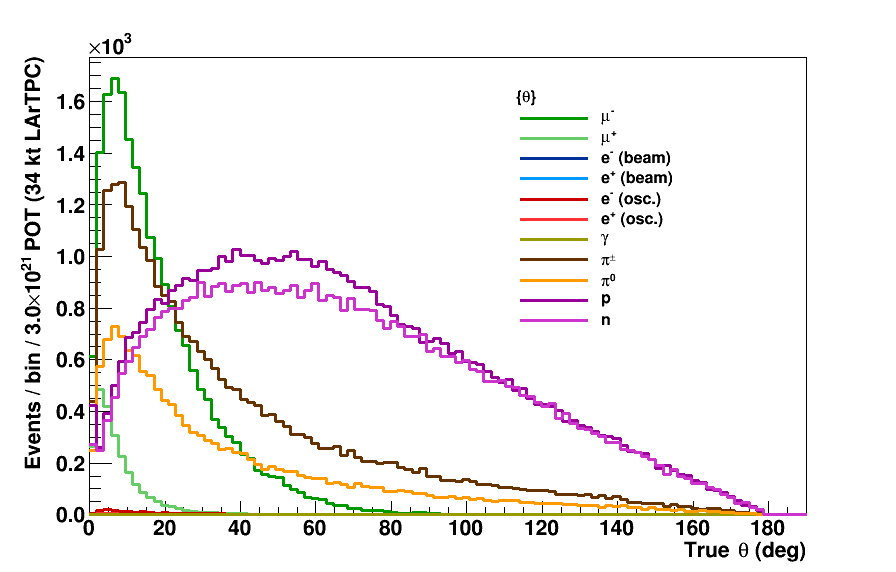
\includegraphics[scale=0.4]{figures/True_theta_per_Particle}
%\label{fig:particle_theta}
%  \caption{Particle angle wrt to the beam axis distributions for particles coming from all fluxes ($\nu_e$, $\nu_\mu$, $\bar \nu_e$ and $\bar \nu_\mu$) at both near and far detector locations.  }
%\end{figure}

%\newpage

DUNE-PT is designed from components that match exactly the DUNE far detector reference design for the first 10~kt detector module.
The test beam detector must be sufficiently large in both
longitudinal and transverse dimensions to contain showering particles up to the energy range of interest ($\sim$10~GeV).
Fig.~\ref{fig:containment} shows the simulated longitudinal and transverse 
energy containment for proton showers up to 10~GeV in energy.
For 10 GeV showers, more than 95\% of the energy is contained in a detector of longitudinal size of 6~m and 
radius of 2.5~m. Showers from pions, kaons, and electrons have also been studied and similar or better containment is achieved in those cases, given the above detector dimensions.
\begin{figure}[htp]
  \centering
  \begin{tabular}{ccc}
%    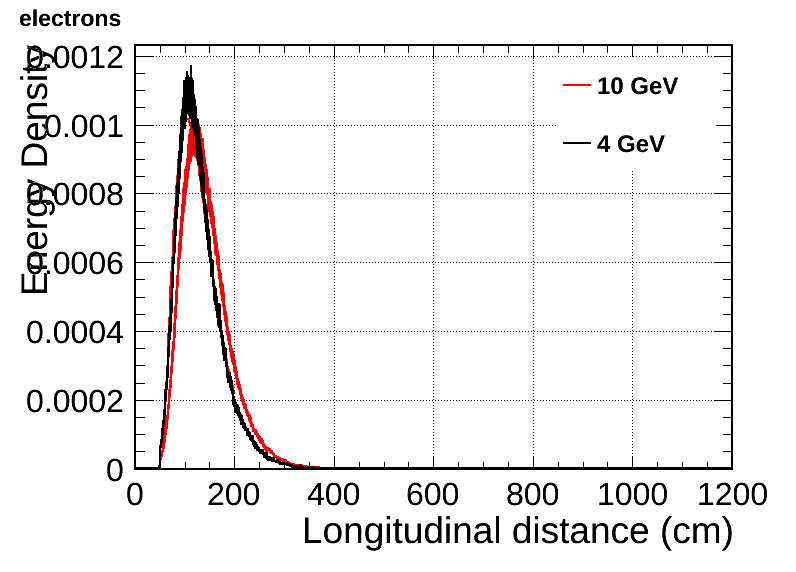
\includegraphics[scale=0.15]{figures/electrons_density_overlay}&
%    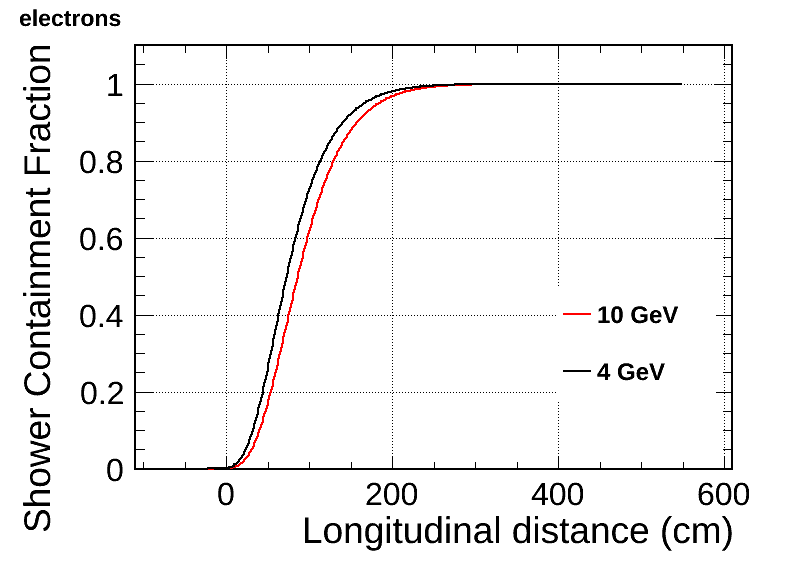
\includegraphics[scale=0.15]{figures/electrons_lcont_overlay}&
%    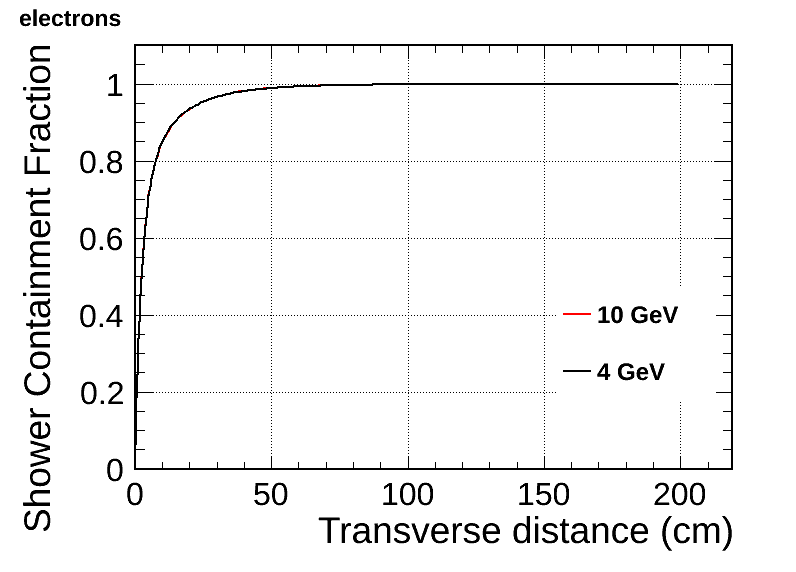
\includegraphics[scale=0.15]{figures/electrons_wcont_overlay}\\
%  
%    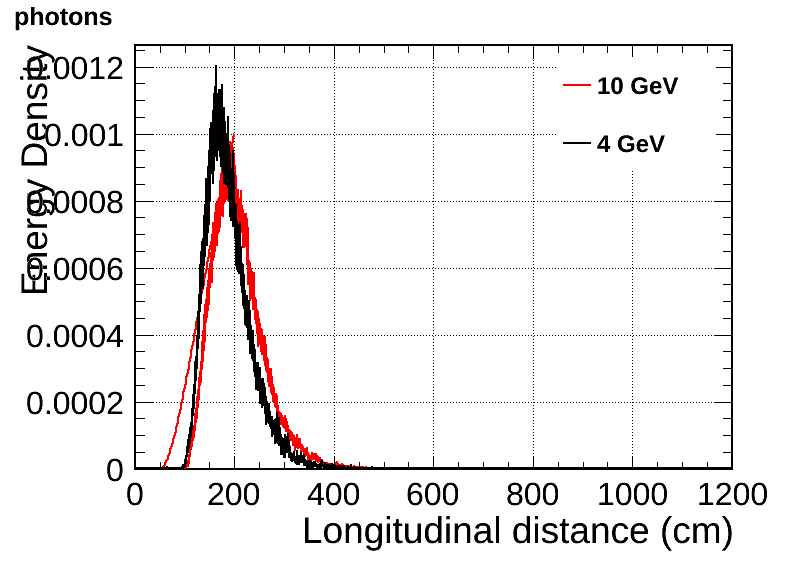
\includegraphics[scale=0.15]{figures/photons_density_overlay}&
%    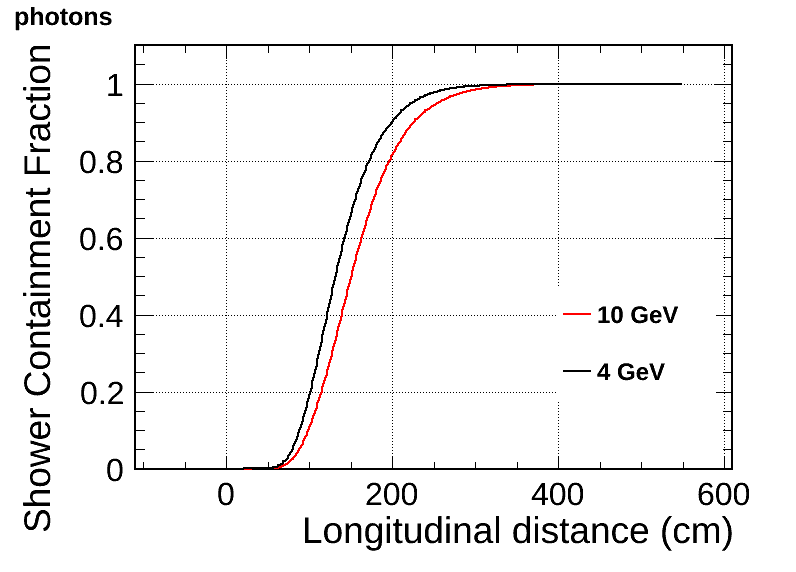
\includegraphics[scale=0.15]{figures/photons_lcont_overlay}&
%    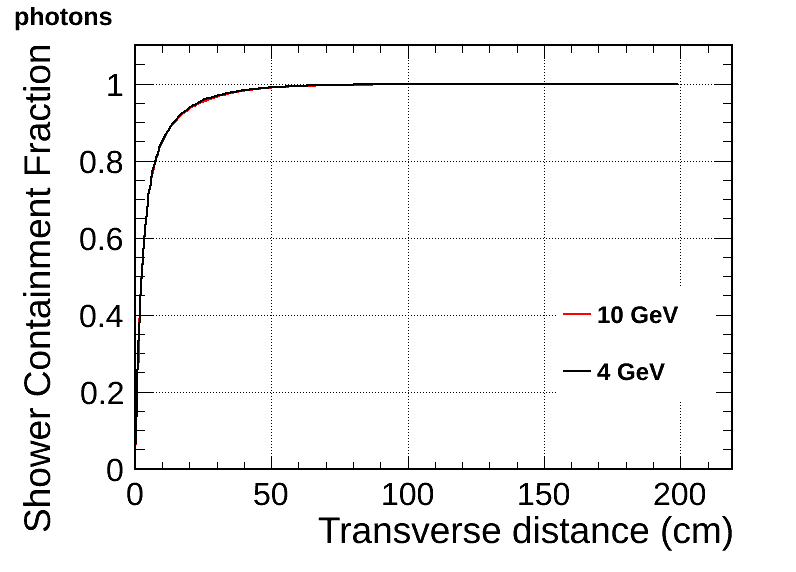
\includegraphics[scale=0.15]{figures/photons_wcont_overlay}\\
%%
%   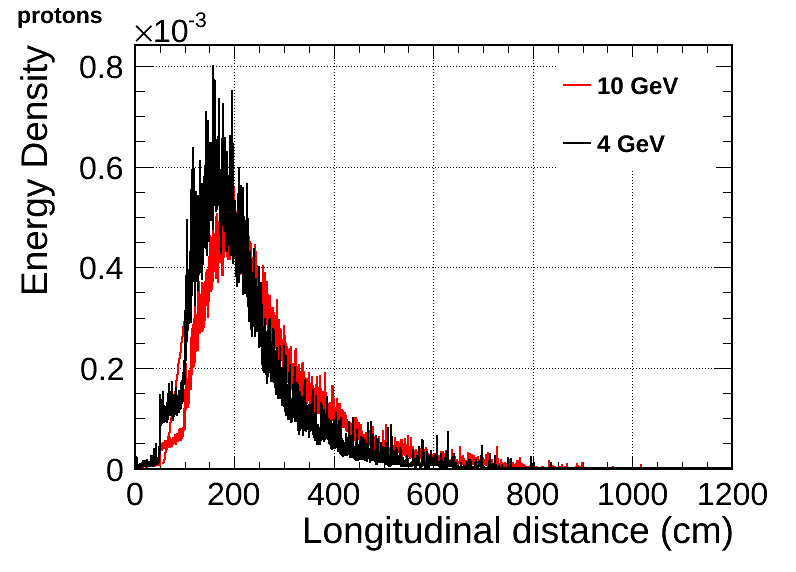
\includegraphics[width=0.31\textwidth,height=3.9cm]{figures/protons_density_overlay}&
   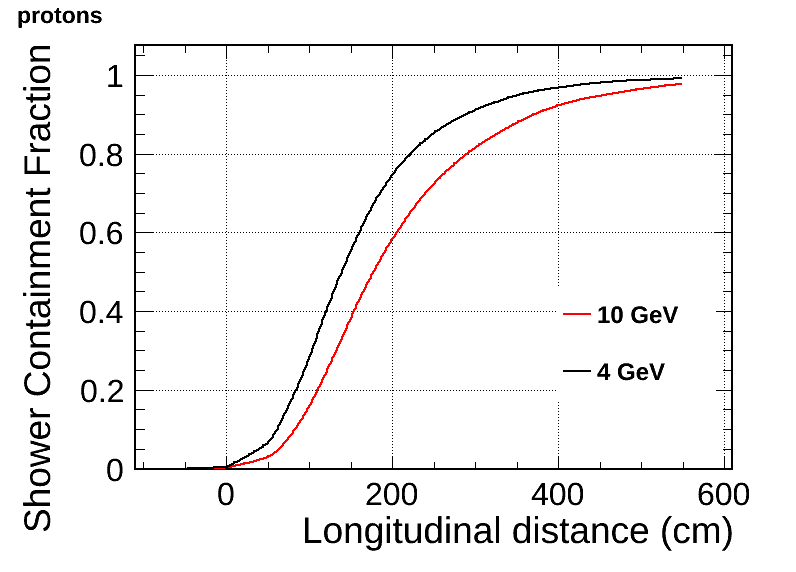
\includegraphics[width=0.49\textwidth,height=4.9cm]{figures/protons_lcont_overlay}&
   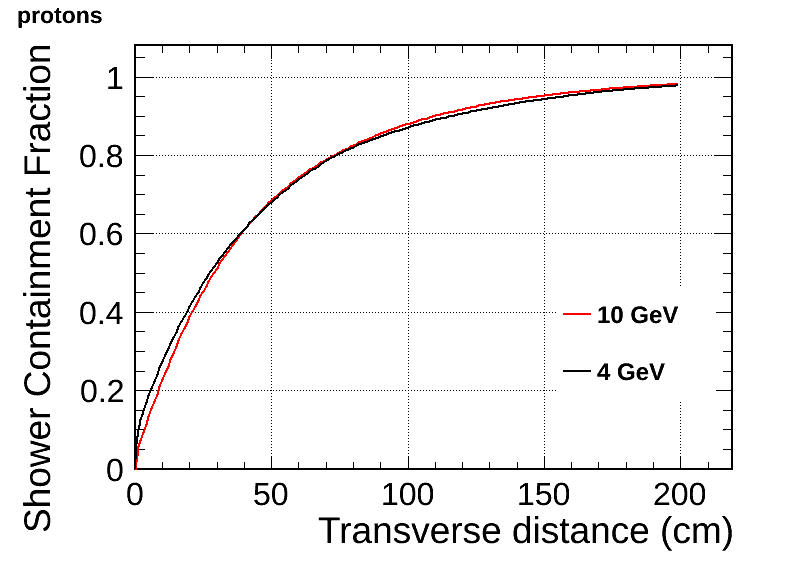
\includegraphics[width=0.49\textwidth,height=4.9cm]{figures/protons_wcont_overlay}\\
%    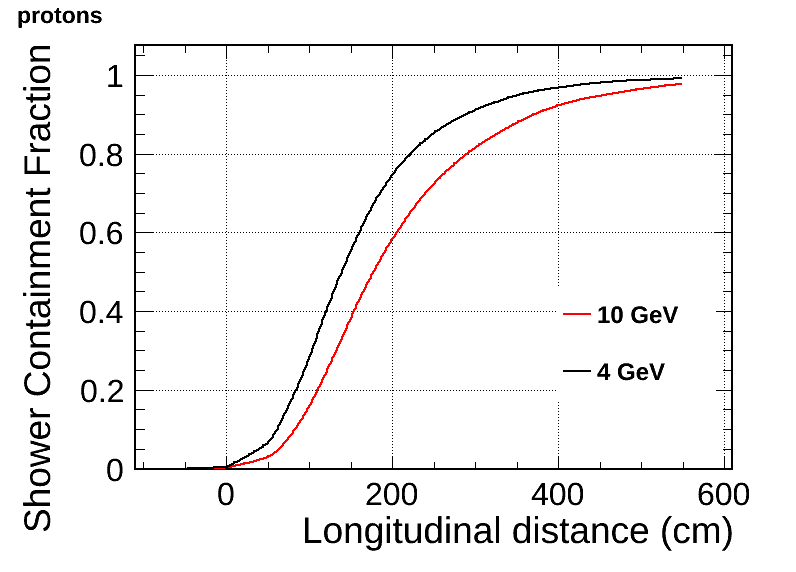
\includegraphics[scale=0.15]{figures/protons_lcont_overlay}&
%    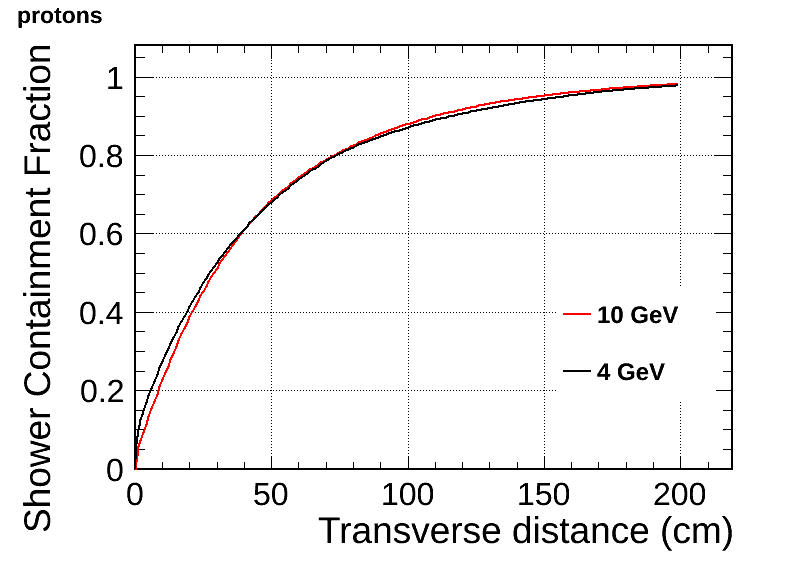
\includegraphics[scale=0.15]{figures/protons_wcont_overlay}\\
% 
%    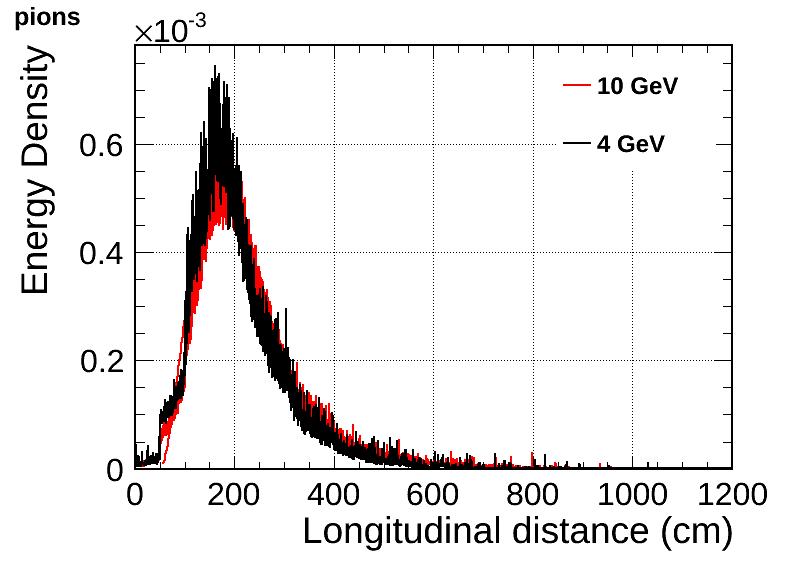
\includegraphics[scale=0.15]{figures/pions_density_overlay}&
%    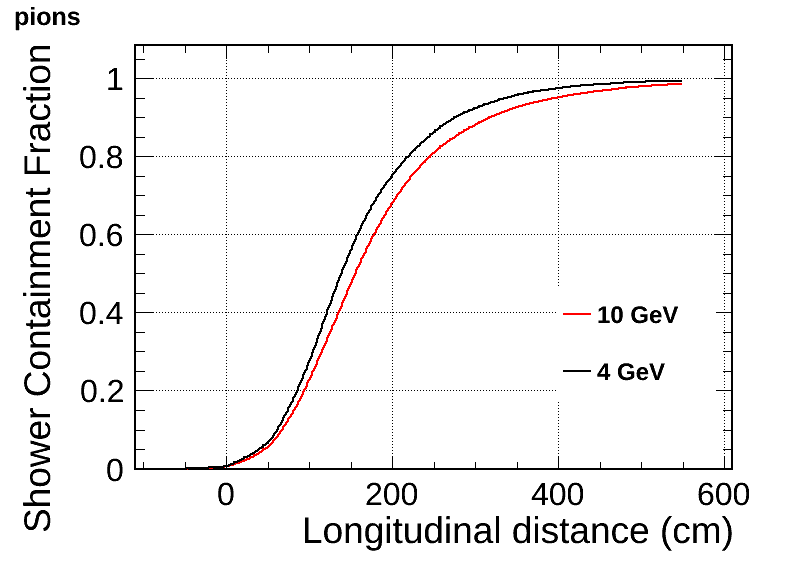
\includegraphics[scale=0.15]{figures/pions_lcont_overlay}&
%    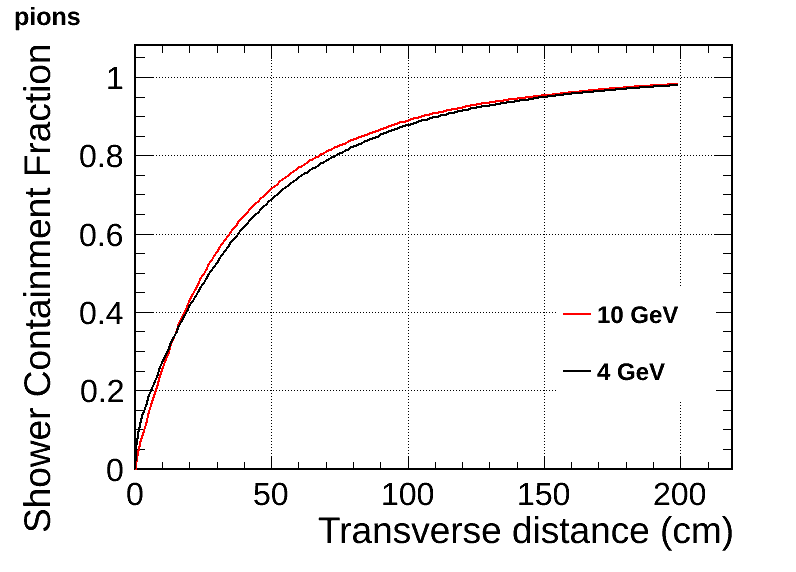
\includegraphics[scale=0.15]{figures/pions_wcont_overlay}\\
 
%   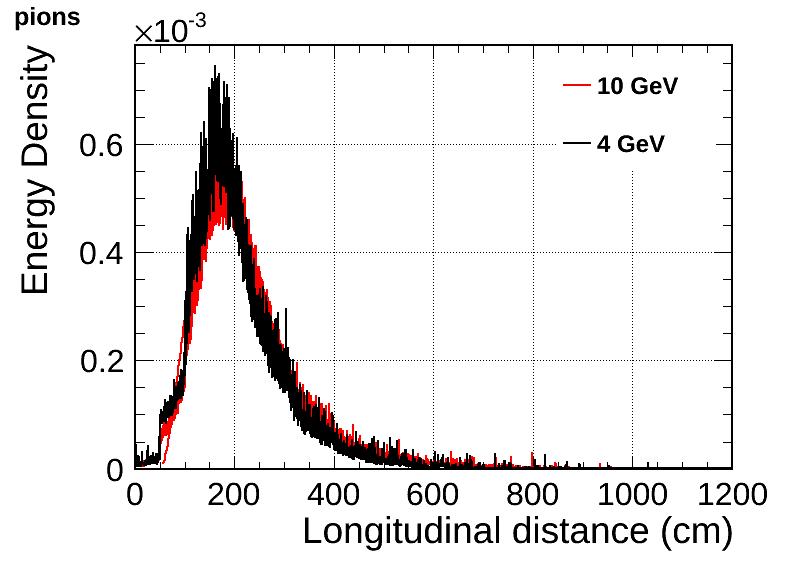
\includegraphics[width=0.31\textwidth,height=3.5cm]{figures/pions_density_overlay}&
%   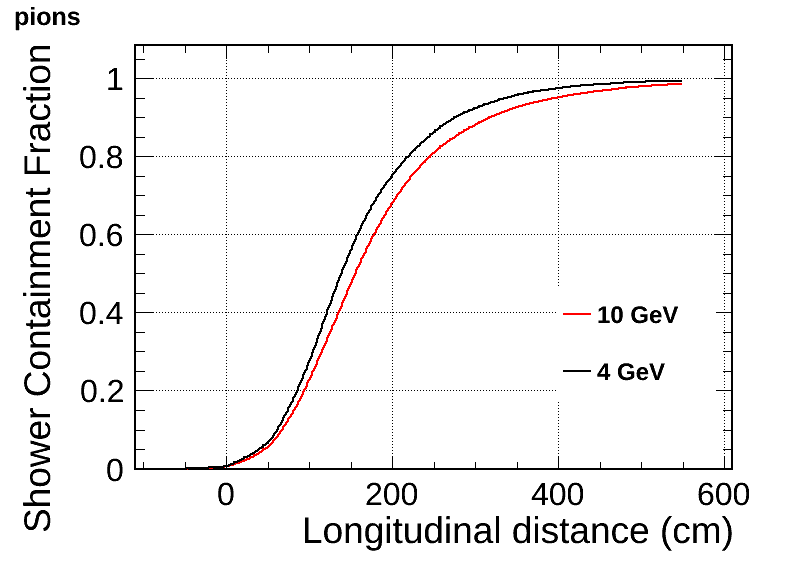
\includegraphics[width=0.31\textwidth,height=3.5cm]{figures/pions_lcont_overlay}&
%   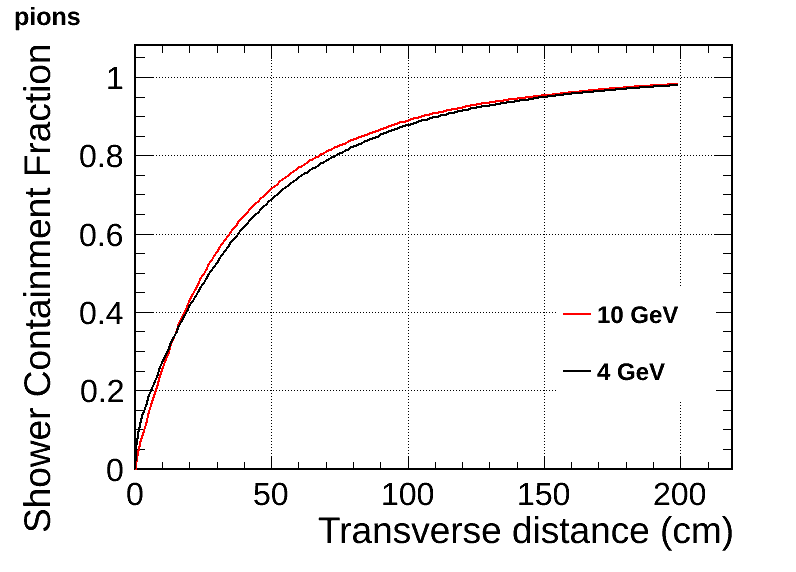
\includegraphics[width=0.31\textwidth,height=3.5cm]{figures/pions_wcont_overlay}\\
%    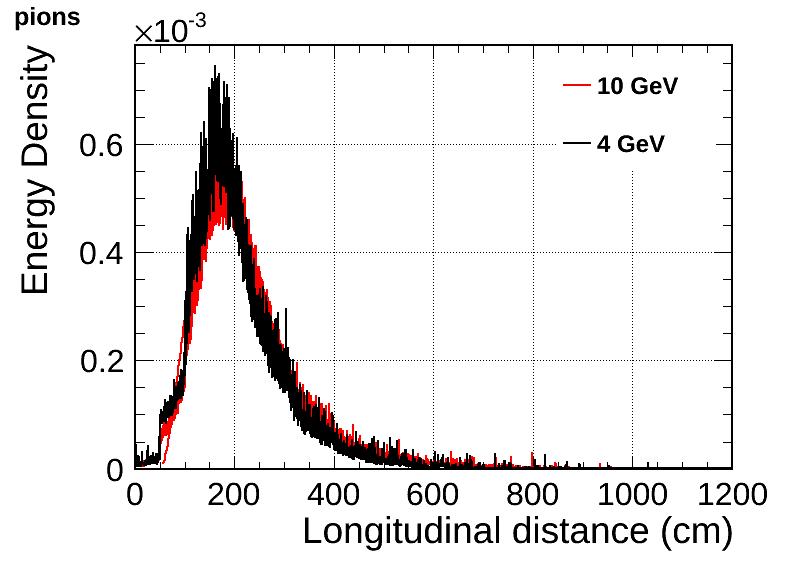
\includegraphics[scale=0.15]{figures/pions_density_overlay}&
%    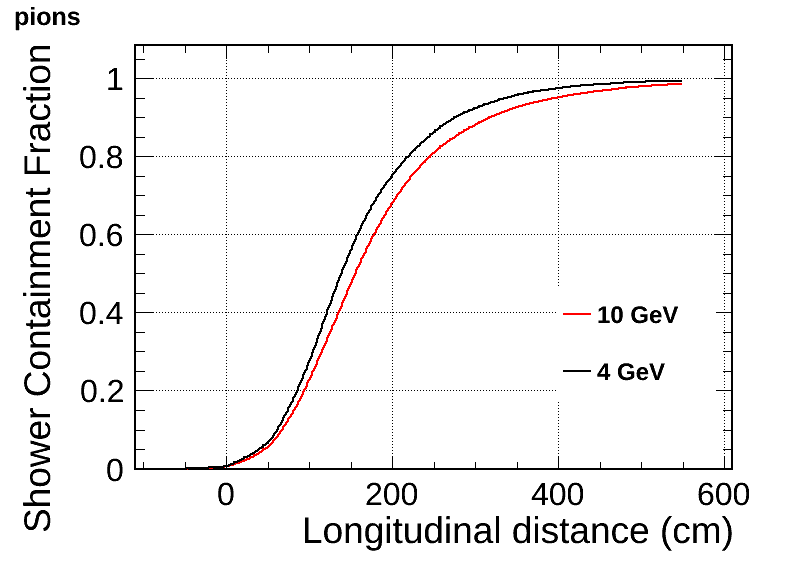
\includegraphics[scale=0.15]{figures/pions_lcont_overlay}&
%    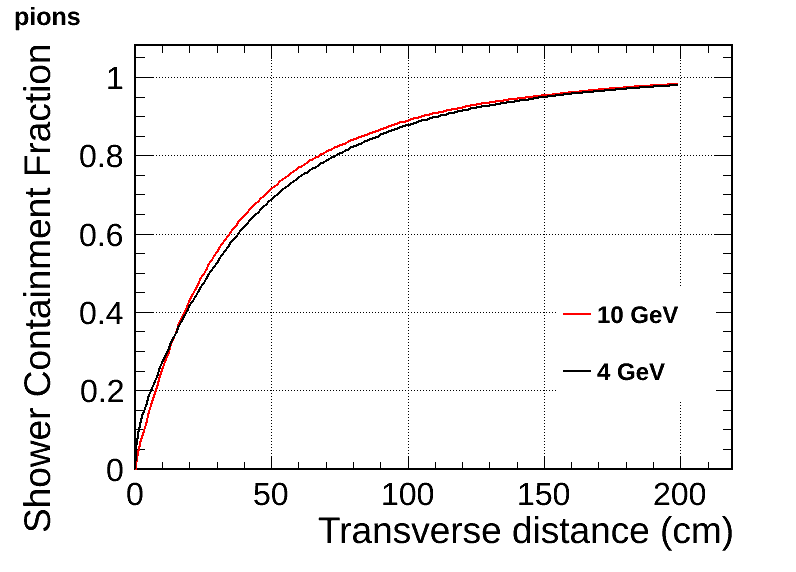
\includegraphics[scale=0.15]{figures/pions_wcont_overlay}\\
 
% 
%    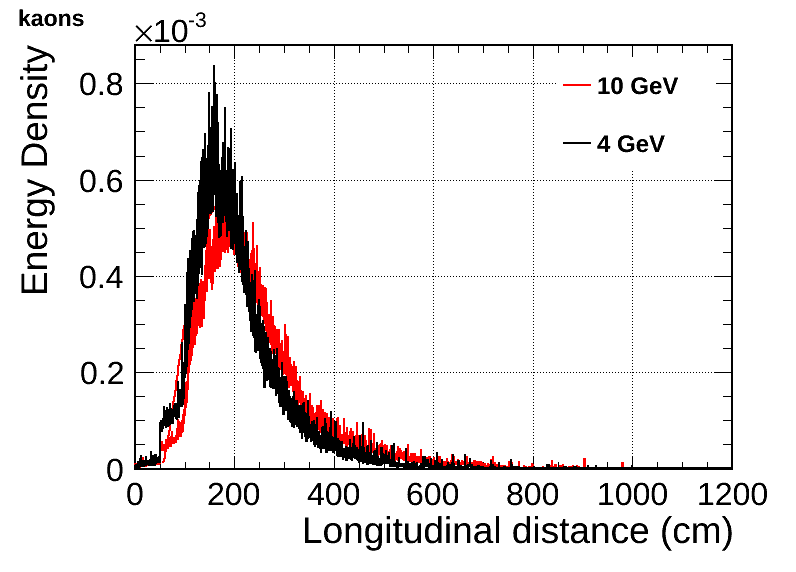
\includegraphics[scale=0.15]{figures/kaons_density_overlay}&
%    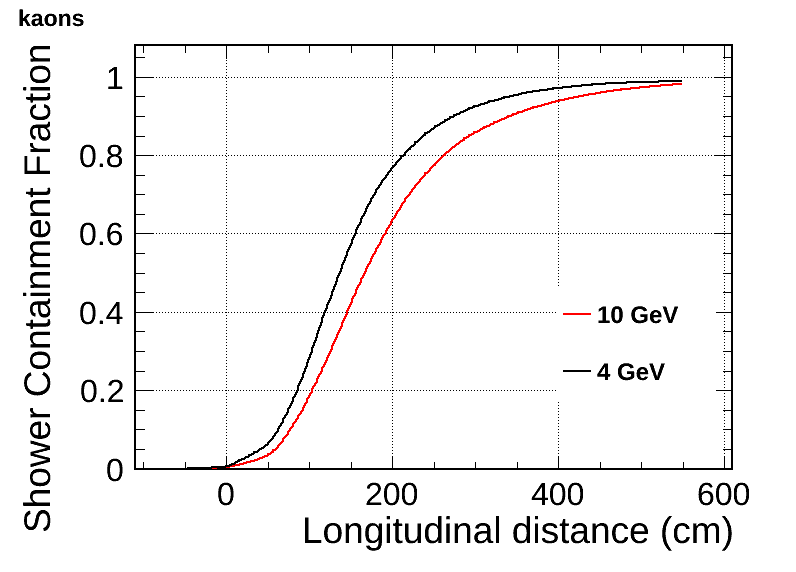
\includegraphics[scale=0.15]{figures/kaons_lcont_overlay}&
%    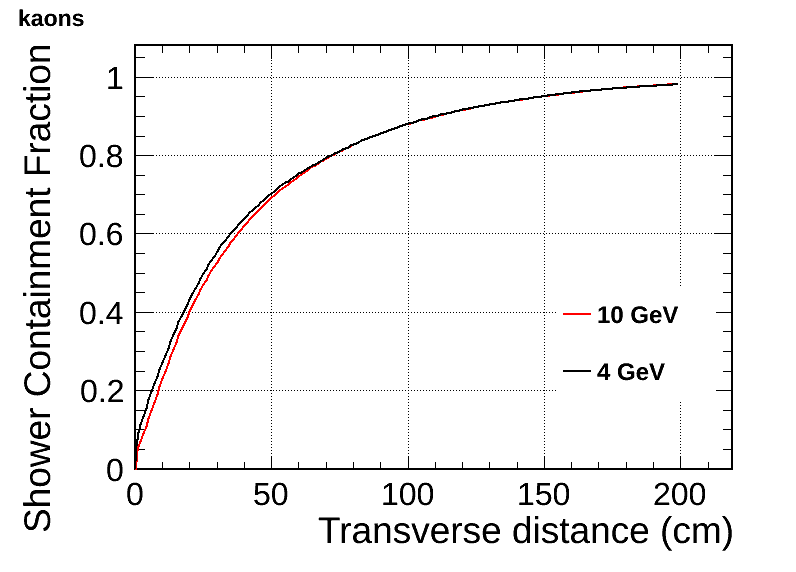
\includegraphics[scale=0.15]{figures/kaons_wcont_overlay}\\
 
  \end{tabular}
  \caption{Simulated longitudinal and transverse containment for proton showers of 4 and 10~GeV/c momenta.
%{\color{red}
%Improve or perhaps remove far left plot (binning too fine).
%Add info on simulation details and containment defn (T. Junk).
%}
}
  \label{fig:containment}  
%For 10 GeV showers, more than 95\% of the energy is contained in a detector of longitudinal size of 550~cm and 
%radius of 200~cm.}
\end{figure}

%\clearpage
%\subsubsection{Particle rates}
%\label{detbeam_rates}
%Estimation of  beam particles rates  necessary to collect high enough statistics in a reasonable time to obtain goals of of the measurements.
% THis should be discussed in the beam section
\subsection {Beam particle requirements}

Table~\ref{tab:runsum} summarizes the requested particle types and momenta along with 
required sample sizes for the test beam program.
\begin{table}[h]
\centering
\begin{tabular}{|c|c|c|l|}
\hline
Particle & Momenta (GeV/c) & Sample & Purpose \\ 
 &  &  Size &  \\ \hline \hline
$\pi^+$       & 0.2, 0.3, 0.4, 0.5, 0.7, 1, 2, 3, 5, 7     &  10k  & hadronic cal, $\pi^0$ content \\ \hline
$\pi^-$       &  0.2, 0.3, 0.4, 0.5, 0.7, 1     &  10k  & hadronic cal, $\pi^0$ content \\ \hline
$\pi^+$   &  2  &  600k & $\pi^o$/$\gamma$ sample \\ \hline
%$\pi^+$ &   1 \& 2  &  10K  & vary angle ($\times$5), reco \\ \hline
proton &  0.7, 1, 2, 3   &  10k & response, PID \\ \hline
proton &  1   &  1M & mis-ID, PD, recombination \\ \hline
e$^+$ or e$^-$       &    0.2, 0.3, 0.4, 0.5, 1, 2, 3, 5, 7        &    10k   & e-$\gamma$ separation/EM shower     \\ \hline
% e$^+$ or e$^-$  &  1 \& 2  &  10K  & vary angle($\times$5), reco \\ \hline
%e$^+$ or e$^-$   (w/rad) &  3  &  20K  & tagged photons \\ \hline
$\mu^-$  &   (0.2), 0.5, 1, 2  &  10k & $E_\mu$, charge sign \\ \hline
$\mu^+$ &   (0.2), 0.5, 1, 2   &  10k & $E_\mu$, Michel el.,charge sign  \\ \hline
$\mu^-$ or $\mu^+$ &   3, 5, 7  &  5k & $E_\mu$ MCS \\ \hline
%$\mu^-$ or $\mu^+$  &  1 \& 2  &  5K  & vary angle ($\times$5), reco \\ \hline
%proton &  1 \& 2 &  10K & vary angle ($\times$5), reco \\ \hline
anti-proton &  low-energy tune  &  (100) & anti-proton stars \\ \hline
K$^+$  & 1 & (13k)   &   response, PID, PD  \\ \hline
K$^+$  & 0.5, 0.7 & (5k)   &   response, PID, PD  \\ \hline \hline
$\mu$, e, proton  & 1 (vary angle $\times$5) & 10k  & reconstruction  \\ \hline
\end{tabular}
\caption{Requirements summary for particle types and momenta.
The sample size column indicates the number of particles for each momentum point.
Items in parenthesis indicate lower priority (see text).
}
\label{tab:runsum}
\end{table}


Pions and protons spanning the energy range expected in DUNE beam neutrino interactions will be used 
primarily to study hadronic shower reconstruction and calibration as described in Sec.~\ref{sec:showers}
 as well as particle identification (PID) algorithms discussed in Sec.~\ref{detbeam_pid}. A sample of 600k
 2~GeV $\pi^+$ will be used to study  secondary $\pi^o$ over a large angular range 
to tune and calibrate electron/photon separation algorithms (see Sec.~\ref{sec_egam}).
A large sample (10$^{6}$) of 1 GeV protons represents a sample of low energy stopping protons over a 
wide angular range needed to study angular
dependent effects on collected charge as described in Sec.~\ref{sec_angle}.
Electrons will be used to benchmark and tune  electron/photon separation algorithms and to calibrate 
electromagnetic showers as discussed in Sec. \ref{sec_egam}.
Muon (and anti-muon) samples are needed to study reconstruction and PID calibration.
Associated samples of Michel electron events will be used to calibrate  
algorithms for charge-sign determination (see Secs.\ref{sec_reco} and \ref{sec_other}).

Charged-kaon samples will be useful to characterize kaon PID efficiency for proton decay sensitivity but
may be hard to obtain.
The anti-proton sample
will be helpful for exotic physics sensitivity studies. Both of these lower priority requests are discussed
in Sec.~\ref{sec_other}.

%Charged pion samples will be used to characterize hadronic shower response and to measure
%absorption cross section parameters on argon.
%for all energies except 0.1 GeV point). 
%Muon samples will be used for calibration and 
%reconstruction tests. Electron samples will be used to measure EM shower response  
%and to tune PID algorithms (statistics shown will far exceed 1\% uncertainty on the mean for 
%EM showers with resolution on the order of 1\% as measured in DOCDB 9434 and 8835. 100k Electron event samples will allow
%high statistics studies of e-gamma separation).  
%Proton response will be studied for reconstruction and to tune PID 
%algorithms. Kaon data will be needed to tune proton decay backgrounds .
%Special runs at various angles with $\pi$, $\mu$, p and electrons will be performed to study reconstruction and tune PID algorithms. 

\subsection{Detector physics validation tests}

%The prototype detector will allow to study the detector response to charge particles from the test beam. 
The measured energy deposition for various particles and its dependence on the direction of the particle will be used to tune
Monte Carlo simulations and allow improvements to reconstruction of neutrino energy and interaction topologies. % with good particle identification.
Measurements of the response to charged particles and
photons with the DUNE-PT will extend and be complementary to
measurements made with other smaller detectors, such as LArIAT \cite{LArIAT}
and CAPTAIN~\cite{captain}.

\subsubsection{Shower calibration}
\label{sec:showers}

Accurate measurement of neutrino energy will require reconstruction of both electromagnetic and hadronic showers. Reconstruction of hadron energy 
in these energy ranges will require knowledge of the fate (interact, decay, or stop) of the
initiating hadron ($\pi^{+/-}$, $p$, or $K^{+/-}$).
%fate (interact, decay, or stop). 
For the case of  interacting hadrons the composition of secondaries
will need to be determined to characterize the response. 
These will include neutrals and particles which 
deposit energy electromagnetically ($\pi^o$, $\gamma$), as well as
secondary hadrons.
%and their energy responses 
The test beam with known incoming particle type and momentum will be used
to characterize interacting hadrons in this energy range.
%quantify responses to initiating hadrons
%($\pi^{+/-}$, $p$, or $K^{+/-}$)
%Hadronic showers initiated by protons in this energy range require

Fig.~\ref{fig:hadronshwr} shows the fraction of true energy deposited by interacting protons with 1~GeV/c (left) and
3~GeV/c (right) incident momenta simulated using FLUKA particle transport code~\cite{fluka05}. 
Interacting protons (65\% of the 1~GeV/c sample) are selected.
% The remaining 
%35\% which range out are be used to study particle identification algorithms (PID) (see Sec.~\ref{detbeam_pid}). 
%Reconstruction is performed with ICARUS spatial and calorimetric reconstruction algorithm~\cite{icarus_reco}.
For this study, visible energy is summed using hit information with corrections applied for the lifetime of 
the drift electrons (No attempt is made to correct for recombination effects or electromagnetic shower fractions). 
The resulting energy deposition in the two cases cannot be 
accurately characterized by an average shower calibration factor. Monte Carlo simulations of 
outgoing particles, especially at low energies, must be checked and bench-marked against calibration data to avoid
large uncertainties from shower modeling. 
\begin{figure}[h!]
  \centering
%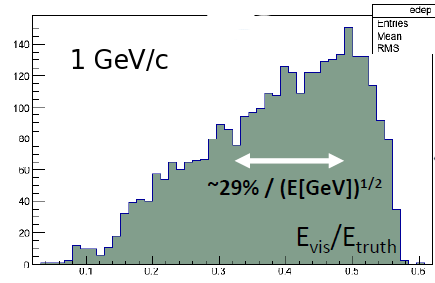
\includegraphics[width=0.49\textwidth,height=5.0cm]{figures/protons_1gev_v0}
%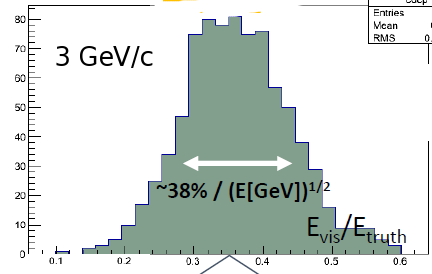
\includegraphics[width=0.49\textwidth,height=5.0cm]{figures/protons_3gev_v0}
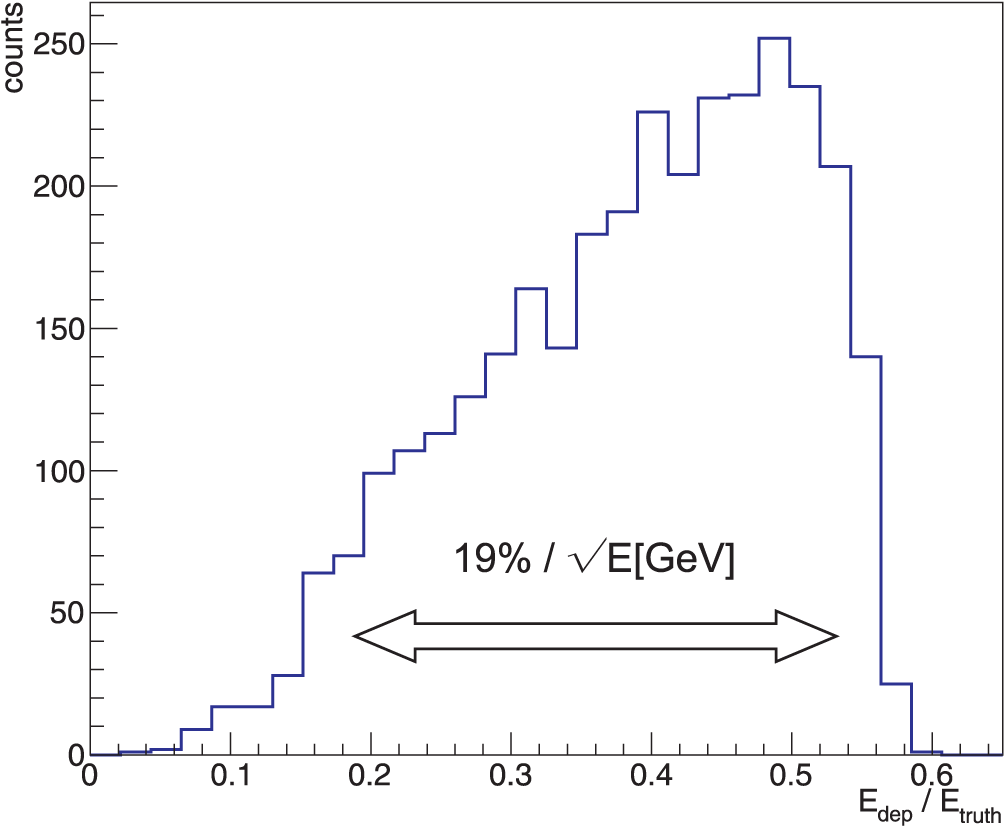
\includegraphics[width=0.49\textwidth,height=5.0cm]{figures/pr1GeV_v2a}
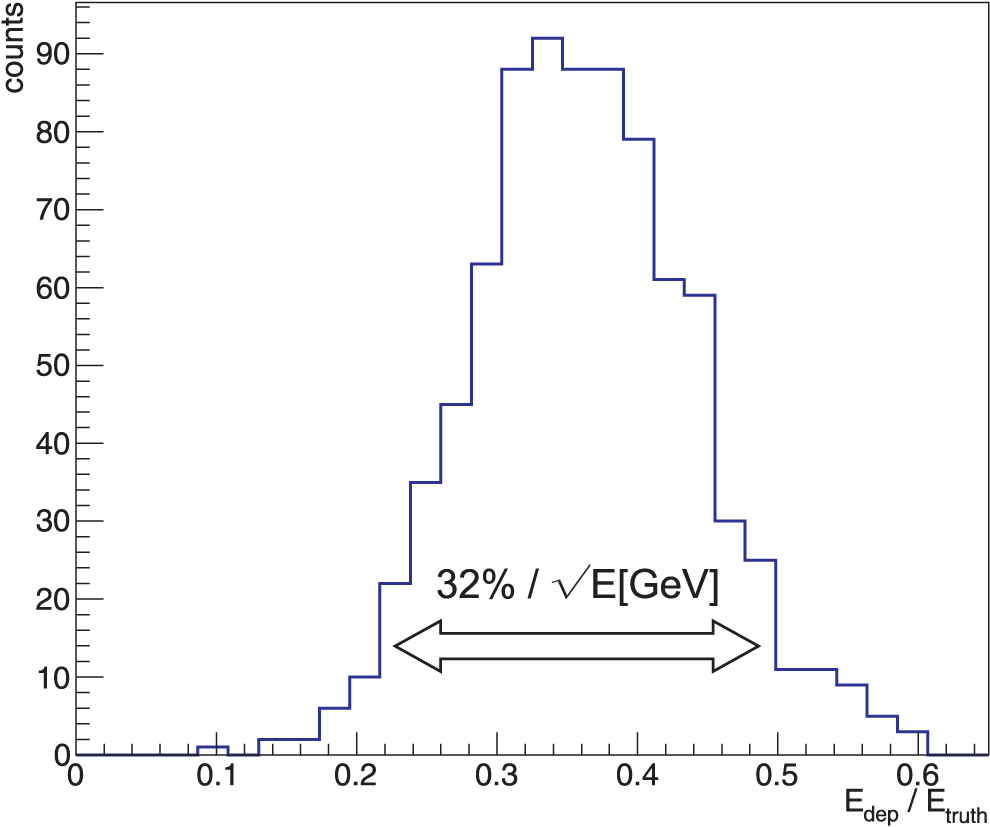
\includegraphics[width=0.49\textwidth,height=5.0cm]{figures/pr3GeV_v2a}
  \caption{Fraction of true energy deposited by interacting protons of 1~GeV/c (left) and
3~GeV/c (right) momenta simulated using FLUKA~\cite{fluka05}.
}
\label{fig:hadronshwr}
\end{figure}

Pion showers at low energies will also be important both for determining the interacted neutrino energy as well
as for modeling neutral current backgrounds resulting from $\pi^o$ content in showers. Significant
 differences in energy deposited in interactions initiated
by $\pi^+$ versus $\pi^-$  are present up to momenta on the order of 1~GeV/c due to different
final state particles and interaction cross sections. This is illustrated in 
Fig.~\ref{fig:pionshwr} which shows the differences in mean energy deposited (left) and width (right) 
for interacting pions ranging from 0.2~GeV/c up to 5~GeV/c momenta.
% simulated using FLUKA~\cite{fluka05}.
Resulting shower calibrations and reconstruction will differ and therefore each charge must be 
studied separately.

\begin{figure}[h!]
  \centering
%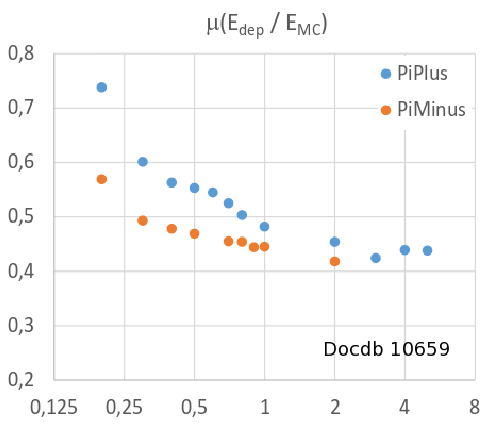
\includegraphics[width=0.49\textwidth,height=5.0cm]{figures/pi+pi-_means}
%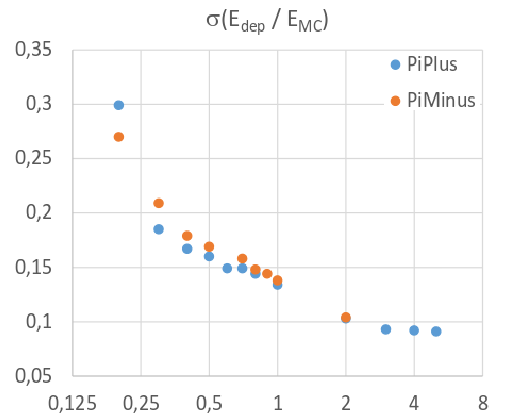
\includegraphics[width=0.49\textwidth,height=5.0cm]{figures/pi+pi-_sig}
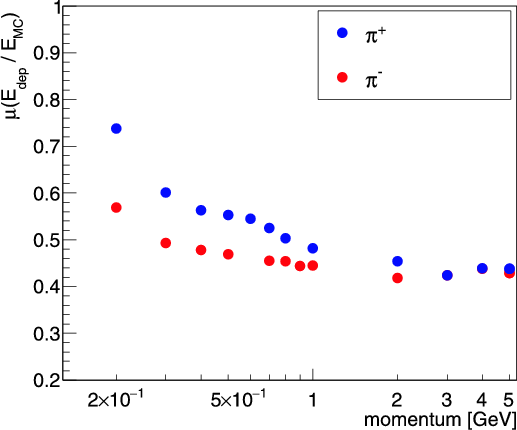
\includegraphics[width=0.49\textwidth,height=6.0cm]{figures/pipimean_ticks1}
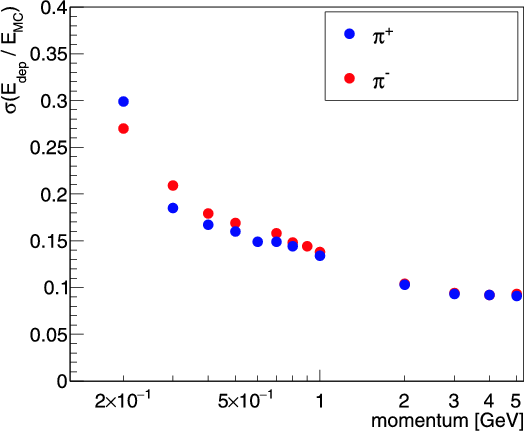
\includegraphics[width=0.49\textwidth,height=6.0cm]{figures/pipisigma_ticks1}
  \caption{Differences in mean energy deposited (left) and width of visible energy (right) 
for interacting $\pi^+$ versus $\pi^-$ ranging from 0.2~GeV/c up to 5~GeV/c. 
}
\label{fig:pionshwr}
\end{figure}


% 
%\begin{table}[h]
%\centering
%\begin{tabular}{|c|c|c|}
%\hline
%Particle     & Momenta (GeV)                                                                                       & Exposure/bin (total)  \\ \hline
%$\pi ^+ $   & 0.2-1.0 (100MeV bins), 1.0-10.0 ( 200MeV bins)    &  1000 (48k)     \\ \hline
%$\pi ^- $    & 0.2-1.0 (100MeV bins), 1.0-10.0 ( 200MeV bins)    &  1000 (48k)     \\ \hline
%$e^+$       & 0.2-10  (100MeV bins), 1.0-10.0 ( 200MeV bins)    &  1000 (48k)       \\ \hline
%$e^- $       & 0.2-10  (100MeV bins), 1.0-10.0 ( 200MeV bins)    &  1000 (48k)       \\ \hline
%$\mu^+$   & 0.2-1.0 (100MeV bins), 1.0-10.0 ( 200MeV bins)    &  1000 (48k)     \\ \hline
%$\mu^-$    & 0.2-1.0 (100MeV bins), 1.0-10.0 ( 200MeV bins)    &  1000 (48k)     \\ \hline
%$p$          &  0.2-1.5 (100MeV bins), 1.5-10.0 ( 200MeV bins)    &  1000 (56k)     \\ \hline
%$\bar p$   &  0.2-1.5 (100MeV bins), 1.5-10.0 ( 200MeV bins)    &  1000 (56k)     \\ \hline
%$K^+$      &  0.2-1.5 (100MeV bins), 1.5-10.0 ( 200MeV bins)    &  1000 (56k)     \\ \hline
%$K^- $      &  0.2-1.5 (100MeV bins), 1.5-10.0 ( 200MeV bins)    &  1000 (56k)     \\ \hline
%\end{tabular}\caption{Data sample requirements for shower calibrations.  Currently about 1k particles is assumed per bin to include variations in the shower topologies. Details MC analysis is necessary. }
%\end{table}
%


\subsubsection{Cross section measurements}


Final state pions are produced copiously in neutrino interactions in the energy range 
of interest
and contribute substantially to total visible energy in the interaction.
These particles can re-interact either in the nuclear medium or after emerging from the target nucleus
and substantially change the visible energy deposited in the event. 
The importance of modeling final state pion interactions on reconstructed neutrino energy have 
been recently demonstrated in the NuMI and Booster beam energy ranges~\cite{miniboonefsi, minervafsi}. 

Detailed knowledge of pion-nucleus cross sections in the sub-GeV energy range is required
to tune generators~\cite{genie} to accurately model event visible energy. 
Existing data used to tune the models
cover limited energies ($<$200~MeV) and are primarily on lighter target nuclei~\cite{fsirev}.
% need to check this reference from R. Ransom talk.
The requested $\pi^+$ and $\pi^-$ samples will allow new data samples for measuring
exclusive final state processes over the full relevant energy range and specifically on argon nuclei. 


%\item pion absorption on argon - Kotlinski, EPJ 9, 537 (2000)
%\item pion cross section as a function of A - Gianelli PRC 61, 054615 (2000)

%There is not currently a satisfactory theory describing absorption. The Valencia group (Vicente-Vacus NPA 568, 855 (1994)) developed model of    the pion-nucleus reaction with fairly good agreement, although not in detail. The actual  mechanism of multi-nucleon absorption
% is not well understood. 
 


\subsubsection{Angular dependence}

\label{sec_angle}

%Ionization charge deposited by charged-particles in the LAr TPC must be calibrated to
%account for recombination effects. 

An angular dependent track correction must be
%Track angle must be accounted for and a correction
applied to deposited charge to accurately calibrate
dE/dx that is used for track momentum and particle ID (see Sec.~\ref{detbeam_pid}). 
An additional angular dependent effect could be present 
due to charge recombination. 
% effects could also be angular dependent. 
%It this is the case
%this will introduce a component that is currently not modeled. 
For example, Jaffe columnar recombination model~\cite{jaffe,argoneut_angle} predicts 
angular dependence given by 
$$Q \approx \frac{Q_o}{1+k_c (dE/dx) / {\cal E} \sin\phi}, $$ 
where
%Recombination modeling 
$Q_o$ and $Q$ are the ionization charge and the collected charge respectively, 
%$dE/dx$ is range based stopping power.
$k_c$ is a constant that depends on LAr diffusion and mobility coefficients, $\cal E$ 
is the electric field strength, and $\phi$ is the angle relative to the drift direction.
%
ICARUS~\cite{icarus_recombination} and LArSoft default recombination models do not currently incorporate angular dependence. 
%(ArgoNeuT~\cite{arogneut_angle} suggests a 
%modified Box model with explicit angular dependence can be incorporated 
%into Birk's law  by replacing ${\cal E}$  with ${\cal E} \sin\phi$).
Recent results from ArgoNeuT~\cite{argoneut_angle} find a small unmodeled
angular dependence in a data sample obtained using stopping protons from 
neutrino interactions in the range 50-300 MeV with angles in the range 40-90$^{\circ}$.

Additional data covering a large angular range would be useful to further investigate angular dependence.
The large sample of 1~GeV protons requested will also be used to study this using 
samples of secondary stopping protons produced in showers at a range of angles with
respect to the field direction.

\subsubsection{Bethe-Bloch parametrization of charged particles and PID}

%
\label{detbeam_pid}

%The reconstruction of events in the LAr TPC is still a challenge but rapid progress has been achieved in recent years (cite pandora and other reconstruction algorithms). Despite the progress reconstruction algorithms have to rely Monte Carlo predictions which don't simulate liquid argon detectors responses correctly. Reconstruction algorithms will benefit greatly from test beam data particularly from the full scale prototype. The reconstruction algorithms will be trained to correctly reconstruct track, electromagnetic and hadronic showers.
%The data of tracks and showers can be used to create a library of reference events with which to tune algorithms.
%which can be sed for matching with he neutrino data, similar to the  LEM (library event matching).

Information on range and charge deposition for stopping charged-particles can be used to 
accurately identify particle type as well as measure kinetic energy. 
Fig.~\ref{fig:resrange}  (left) shows track energy loss per unit length\footnote{Signal attenuation due to recombination effect is not corrected for the PID purpose since it is a deterministic transformation which does not add measurement information.}
(dQ/dx) as a function of residual 
track range for simulated muon, pion, proton and kaon particle tracks. 
A neural-net-based algorithm~\cite{nn_pid,rd_pid}
was used to determine PID functions for each particle hypothesis.
% at a bin centered at 6$\pm$1~cm.
%  for each particle hypothesis.
%functions for each particle hypothesis. 
Fig.~\ref{fig:resrange} (right) 
shows the distribution of reconstructed dQ/dx in a narrow bin of residual range 6($\pm$1)cm to illustrate the scale of difference between particle types. Proton and kaon bands are well separated from each other and from pion and muon bands, while pion and muon bands are almost overlapping which is challenging for the efficient separation. 
Simulation is performed with
FLUKA~\cite{fluka05} and ICARUS geometry (3~mm wire pitch) and reconstruction code~\cite{icarus_reco}.
%Stopping particles were selected using truth information.

%shows the result for events in the residual range bin centered at 6($\pm$1)~cm.
The PID efficiency and purity will  depend on the detector configuration, geometry and 
reconstruction algorithm. The DUNE APA configuration and reconstruction algorithms
%Fig.~\ref{fig:resrange} uses ICARUS geometry with 3~mm pitch, APA configuration 
may give significantly different results, especially for pion/muon separation. 
%Plots were made for 3mm pitch, we don't have such simulation for APA configuration, it may differ a bit (which does not change much for proton/kaon, but can be significant for pion/muon).
It is therefore important to test PID in a realistic prototype detector
data in the presence of all detector effects.
Event samples which include an adequate number of stopping particles for each species
(muon, pions, protons and kaons) are included in the particle summary request in order to 
perform tests of PID algorithms and Bethe-Bloch calibration measurements.


%The tail is used to calibration the MIP response, the region near the end of the track is used
%to give PID information. (WIP)
%Test beam measurements of stopping particles of each type will be used
%to calibrate the energy deposition functions and to determine particle 
%mis-ID probabilities. 
\begin{figure}[h!]
  \centering
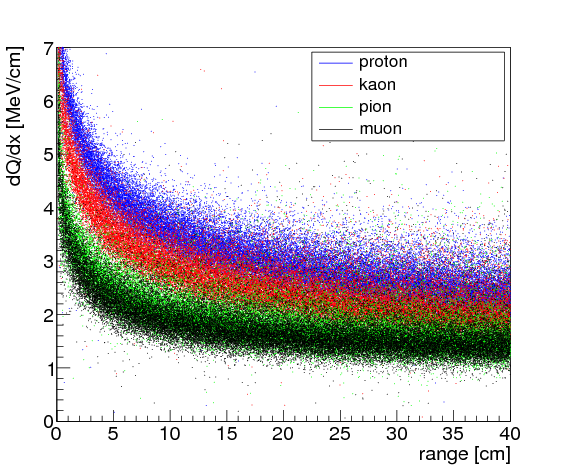
\includegraphics[width=0.53\textwidth,height=6.0cm]{figures/pids_new}
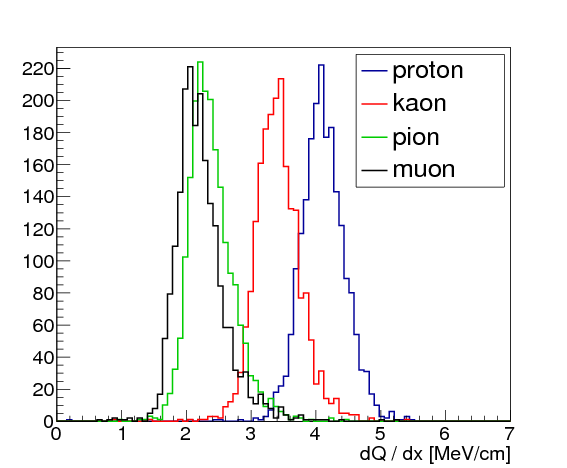
\includegraphics[width=0.46\textwidth,height=6.0cm]{figures/prkpimu_new}
%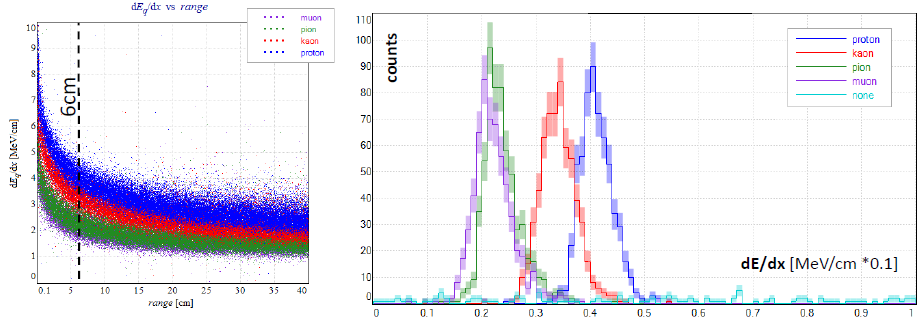
\includegraphics[width=\textwidth,height=5.0cm]{figures/pid_curves}
  \caption{ICARUS simulated track dQ/dx as a function of residual range for muons, pions, protons and kaons, used as training data in a neutral-net-based PID algorithm (left). Distribution of dQ/dx for each particle type for a bin with residual range 
6($\pm$1)~cm (right). The small difference between muon and pion PID is illustrated.
}
\label{fig:resrange}
\end{figure}




%collected particle charge, track angle, as well as 
%which depends strongly 

\subsubsection{Reconstruction effects}
\label{sec_reco}

Reconstruction algorithms use all three wire planes and the drift time for 3D track and event reconstruction. The quality of reconstruction is affected by two main factors that can be quantified with test beam data:
\begin{itemize}
\item The complexity of the event topology, which includes the number of objects overlapping in 2D projections and the number of possible object associations between 2D projections. The topology complexity depends on the energy of the incident particle. Hadronic showers collected with the test beam can provide data sample to assess the reconstruction algorithm performance and test its dependence on the incident particle energy.
\item Orientation of the reconstructed object w.r.t. the readout wires and electron drift direction:
\begin{itemize}
\item Tracks and cascades in the plane parallel or almost parallel to the wire planes have nearly identical hit drift time. These drift times are required for the 3D reconstruction. Under real detector conditions reconstruction algorithms can show varying performance 
 for this class of objects, especially in the presence of noise affecting hit time reconstruction.
\item A 2D projection of objects aligned with the wires of one of the planes is strongly shortened, which limits the amount of information available to the reconstruction algorithm; the two other wire planes can be used for spatial reconstruction.  However, the validation of the correctness of reconstruction, calculated from the 3D object projected to the third plane, is less efficient.
The most important aspect of this issue is the use of all planes for the charge measurement. If the reconstructed object is aligned with collection wires then the calorimetric measurement has to be carried out with the signal from the induction planes. The additional shielding wire plane in the DUNE design will improve the quality of the bipolar induction plane signals.  The test beam 
data will help with the calibration of these signals.
\item Objects aligned with the drift field are projected onto a low
number of wires and have a large span of drift time. The wire signals in these
cases are significantly different than those from tracks at higher angles with
respect to the drift field, and therefore require a dedicated signal processing
algorithm to do hit reconstruction. Corrections for angular dependence of
recombination will also need to be included in the calorimetric reconstruction
and calibrated with real data.
%Objects aligned with the drift field are projected to a low number of wires and have a large span of drift time. Wire signals of such objects are significantly different than those of objects at higher angles w.r.t. the drift field, requiring a dedicated signal processing for the hit reconstruction. In such orientation also the correction of eventual angular dependence of the recombination effect should be included in the calorimetric reconstruction and calibrated with real data.
\end{itemize}
\end{itemize}

%Main issues for the reconstruction algorithms:
%\begin{itemize}
%\item Reconstruction algorithms use all three signal planes for 3D track and event reconstruction. 
%If the orientation of the track/shower is such that it is aligned with wires on one of the planes, it significantly reduces quality of reconstructed objects. 
%\item Calorimetry with collection and induction planes. In the ICARUS experiment the deposited energy was reconstructed from the signal on the collection plane. The induction planes bipolar signal wasn't "stable" enough to use it for calorimetric measurement. In the ELBNF design there is additional shielding  wire plane which will improve the quality of the bipolar signal and the  test beam experiment will help with its calibration.
%\item   Vertexing.
%\item Reconstruction efficiency for low energy particles. The reconstruction algorithm suffer from the lose of efficiency for low energy particle or particles which leave less than 200-300 hits. Training the algorithms on a low energy particles from the test beam will improve the quality and efficiency of the reconstructed objects.
%\end{itemize}

Any reconstruction algorithm will depend on the particular choices in the TPC design. 
Therefore bench-marking our reconstruction algorithms with a prototype of the final design will
be invaluable to understand the performance of reconstruction.

%
%\begin{table}[h]
%\centering
%\begin{tabular}{|c|c|c|}
%\hline
%Particle     & Momenta (GeV)                                                                                       & Exposure/bin (total)  \\ \hline
%$\pi ^+ $   & 0.2-1.0 (100MeV bins), 1.0-10.0 ( 200MeV bins)    &  500 (26.5k)     \\ \hline
%$\pi ^- $    & 0.2-1.0 (100MeV bins), 1.0-10.0 ( 200MeV bins)    &  500 (26.5k)     \\ \hline
%$e^+$       & 0.2-10  (100MeV bins), 1.0-10.0 ( 200MeV bins)    &  500 (26.5k)       \\ \hline
%$e^- $       & 0.2-10  (100MeV bins), 1.0-10.0 ( 200MeV bins)    &  500 (26.5k)       \\ \hline
%$\mu^+$   & 0.2-1.0 (100MeV bins), 1.0-10.0 ( 200MeV bins)    &  500 (26.5k)     \\ \hline
%$\mu^-$    & 0.2-1.0 (100MeV bins), 1.0-10.0 ( 200MeV bins)    &  500 (26.5k)     \\ \hline
%$p$          &  0.2-1.5 (100MeV bins), 1.5-10.0 ( 200MeV bins)    &  500 (27.8k)     \\ \hline
%$\bar p$   &  0.2-1.5 (100MeV bins), 1.5-10.0 ( 200MeV bins)    &  500 (27.8k)     \\ \hline
%$K^+$      &  0.2-1.5 (100MeV bins), 1.5-10.0 ( 200MeV bins)    &  500 (27.8k)     \\ \hline
%$K^- $      &  0.2-1.5 (100MeV bins), 1.5-10.0 ( 200MeV bins)    &  500 (27.8k)     \\ \hline
%\end{tabular}\caption{Data sample requirements for the development of the reconstruction algorithms. The most important are  the low momenta particles where the showers are more likely to have different topologies. }
%\end{table}


\subsubsection{e/$\gamma$ separation}
\label{sec_egam}

The search for a CP violation phase using $\nu_e$ appearance 
in a $\nu_\mu$ beam requires good electron/photon separation.
Backgrounds originating from photons produced primarily from 
final state $\pi^0$'s must be identified and removed from the signal
electron sample. 

High energy photons can undergo two process: pair production and Compton scattering. 
The dominant process for photons with energies of several hundred MeV or more is 
e$^+$ e$^-$ pair production.
%energies. 
%For pair production the 
e/$\gamma$ discrimination
for this process can be achieved using the beginning of the electromagnetic shower, where 
a single MIP is characteristic of electron energy deposition while two MIPs is consistent 
with a photon hypothesis.
In the case where the photon Compton scatters, the two particles cannot easily be distinguished
from the energy deposition pattern.


\begin{figure}[h!]
  \centering
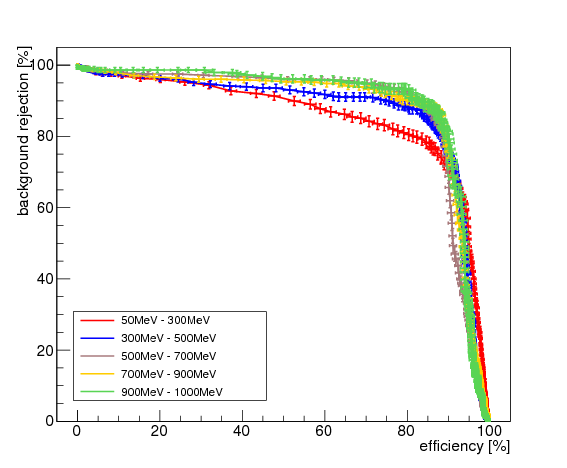
\includegraphics[width=0.49\textwidth,height=6.0cm]{figures/eff-bgdrej-diffen}
%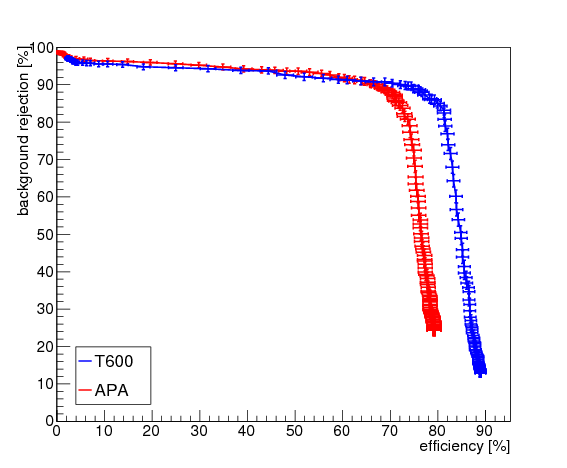
\includegraphics[width=0.49\textwidth,height=6.0cm]{figures/APAT600_all_norm}
  \caption{
 Photon background rejection versus electron identification efficiency for various energies, calculated for and normalized to samples which pass the reconstruction. 
The simulation was performed in APA design configuration (4.67~mm wire pitch, induction wires at $\pm$35.7$^{\circ}$ w.r.t. collection wires). 
}
\label{fig:egam}
\end{figure}
Electron-photon separation has been studied in LAr TPCs
(ICARUS~\cite{icarus_eg} and ArgoNeuT~\cite{argoneut_eg}).
% numbers come from Dorotas plot docdb 10660 
%as shown in Fig.~\ref{fig:egam1}.
%Currently the 
%separation efficiency is estimated to be at the level of of 95 \% (?) 
Fig.~\ref{fig:egam} 
 shows estimated photon background rejection versus electron identification efficiency using 
simulated isotropic electron and photon event samples  with the 
APA geometry configuration ~\cite{dunecdr}.
% and propagated thorough the 
%event reconstruction chain 
The results are found to be mildly dependent
on incoming particle energy in the range of interest. 
%
Our studies indicate that rejection and efficiency depend 
on particular features of the geometry including wire pitch and plane 
orientation which affect the reconstruction. 
For example, a preliminary comparison of signal efficiencies for a simulated 
DUNE APA configuration with the ICARUS T600 geometry
and averaged over the energy range 0.2-1.0 GeV shows 
a 10\% higher efficiency for the 3~mm wire spacing used in ICARUS.
The study does not yet include electron diffusion.
%
Pure samples of electrons and photons in the sub-GeV energy range will be
needed to tune the separation algorithms and to measure 
detector-dependent electron-photon separation efficiency and purity.

%(right) Photon background rejection versus electron identification efficiency
%integrated over the energy range 0.2-1.0 GeV for two different readout designs: APA parameters as on the left plot, ICARUS parameters: 3~mm wire pitch, induction wires at $\pm$60$^{\circ}$ w.r.t. collection wires. 
%Rejection and efficiency values are normalized to the full data sample size, including events which do not pass reconstruction.






\subsection{Other measurements} 
\label{sec_other}

The DUNE experiment will be capable of addressing other physics beyond the long-baseline neutrino measurements with the unique massive underground LAr TPC. Event samples discussed here include those that support this rich array of additional physics goals.
%The DUNE experiment will be capable of addressing other new physics possibilities with its one-of-a-kind
%massive underground LAr TPC. Event samples discussed here include those that support DUNE
%rich array of other physics goals. 


\subsubsection{Supernova and Michel electrons}

Neutrinos produced in supernova burst (SNB) explosions are calculated to be in the few-to-30-MeV range.
The DUNE Far Detector is expected to have unique sensitivity to the $\nu_e$'s from a SNB in our galaxy.
%
The test beam cannot offer a sample of  such low energy electrons, but Michel electrons  produced by 
decaying stopped muons are ideal to calibrate electron response in the appropriate 10-50~MeV energy range. 
The requested sample of low energy muons will supply the 1400 Michel electrons required for a 1\% 
calibration of electrons in this energy range. This sample can be compared to a similar Michel electron sample
stemming from stopping cosmic muons.

%\begin{table}[h]
%\centering
%\begin{tabular}{|c|c|c|}
%\hline
%Particle     & Momenta (GeV/c)    & Exposure/bin  \\ \hline
%$\mu^+$   & (0.2), 0.5, 1      &  10K    \\ \hline
%\end{tabular}\caption{Stopping . }
%\end{table}

\subsubsection{Charge sign determination}

It is not possible to determine the charge of the particle on an event by event basis with non-magnetized LAr TPC detectors. A statistical separation will be studied which will make use of differences in muon versus anti-muon capture cross sections and lifetime.
%However, the statistical analyst will be possible. We will fit the muon's half time which is different for muons and antimony due to different muon capture cross sections. 
For the $\mu^-$ we expect about 99.9\% to be captured on argon whereas essentially all $\mu^+$ decay \cite{stopmu}.
Charge-sign tagged $\nu_\mu$ samples may be useful to constrain exotic possibilities such as
non-standard neutrino interactions which predict differences in the particle and anti-particle survival probabilities. 


\subsubsection{Proton decay sensitivity and background samples}


The DUNE experiment in the deep underground location will seek to detect several modes of proton decay.
In particular, a first ever LAr detector of this scale underground will primarily improve sensitivity to 
proton decays with final state kaons such as  ${p \rightarrow K^+ \overline{\nu}}$. 
Sensitivity to this process is studied in \cite{bueno}. $K^+$ detection efficiency is estimated to be $>$97\% in the
appropriate momentum range (500-800 MeV/c). The kaon samples requested in Table~\ref{tab:runsum} are needed to directly measure 
$K^+$ PID and detection efficiency. 

Obtaining low energy kaons will likely be difficult in this beamline.
A sample of 13k beam kaons with 1~GeV/c momentum are requested to provide 2k stopping $K^+$ track samples for PID studies.
(Only 15\% of $K^+$ stop at 1~GeV/c.)


%\begin{table}[h]
%\centering
%\begin{tabular}{|c|c|c|}
%\hline
%Particle     & Momenta (GeV/c) & Exposure/bin  \\ \hline
%\hline
%K$^+$  &  1 & (13k)    \\ \hline
%K$^+$  & 0.5, 0.7 & (5k)   \\ \hline
%proton &  1  &  (1M)  \\ \hline
%\end{tabular}\caption{Samples related to proton decay physics requirements.}
%\label{pdktable}
%\end{table}

A sizable sample of protons ($\sim 10^6$)
are requested to study the possible background contributions to  $p \rightarrow K^+ \overline{\nu}$.
This sample of  protons are needed to quantify the possibility that an interacting proton 
is  misidentified as stopping kaon. A proton interaction which produces neutrals and one charged pion 
(which is misidentified or subsequently decays to $\mu$) can fake the final state kaon signal.


\subsubsection{Anti-proton annihilation }

A sample of anti-protons would be useful to calibrate the $p$-$\overline{p}$ annihilation process. 
This would provide input to exotic an baryon number violating process in which oscillation between neutron and anti-neutron occurs and results in a
% (reference) modeling of 
subsequent  $n$-$\overline{n}$ annihilation. The modeling of $p-\overline{p}$ annihilation could be
studied and tuned on a low-energy $\overline{p}$ beam sample and used to constrain the related modes 
expected for  $n$-$\overline{n}$ annihilation. These events would be tagged in the 
mixed-mode beam. Events in the sub-GeV range would be the most useful for this purpose.




